%%%%%%%%%%%%%%%%%%%%%%%%%%%%%%%%%%%%%%%%%
% Journal Article
% LaTeX Template
% Version 1.4 (15/5/16)
%
% This template has been downloaded from:
% http://www.LaTeXTemplates.com
%
% Original author:
% Frits Wenneker (http://www.howtotex.com) with extensive modifications by
% Vel (vel@LaTeXTemplates.com)
%
% License:
% CC BY-NC-SA 3.0 (http://creativecommons.org/licenses/by-nc-sa/3.0/)
%
%%%%%%%%%%%%%%%%%%%%%%%%%%%%%%%%%%%%%%%%%

%----------------------------------------------------------------------------------------
%	PACKAGES AND OTHER DOCUMENT CONFIGURATIONS
%----------------------------------------------------------------------------------------

\documentclass[twoside,twocolumn]{article}

\usepackage{blindtext} % Package to generate dummy text throughout this template 

\usepackage[sc]{mathpazo} % Use the Palatino font
\usepackage[T1]{fontenc} % Use 8-bit encoding that has 256 glyphs
\linespread{1.05} % Line spacing - Palatino needs more space between lines
\usepackage{microtype} % Slightly tweak font spacing for aesthetics

\usepackage[english]{babel} % Language hyphenation and typographical rules

\usepackage[left=24mm, right=24mm,top=32mm,columnsep=20pt]{geometry} % Document margins
\usepackage[hang, small,labelfont=bf,up,textfont=it,up]{caption} % Custom captions under/above floats in tables or figures
\usepackage{booktabs} % Horizontal rules in tables

\usepackage{lettrine} % The lettrine is the first enlarged letter at the beginning of the text
\usepackage[table]{xcolor}

\usepackage{enumitem} % Customized lists
\setlist[itemize]{noitemsep} % Make itemize lists more compact

\usepackage{abstract} % Allows abstract customization
\renewcommand{\abstractnamefont}{\normalfont\bfseries} % Set the "Abstract" text to bold
\renewcommand{\abstracttextfont}{\normalfont\small\itshape} % Set the abstract itself to small italic text

\usepackage{titlesec} % Allows customization of titles
%\renewcommand\thesection{\Roman{section}} % Roman numerals for the sections
%\renewcommand\thesubsection{\roman{subsection}} % roman numerals for subsections
\titleformat{\section}[block]{\large\scshape\centering}{\thesection.}{1em}{} % Change the look of the section titles
%\titleformat{\subsection}[block]{\large}{\thesubsection.}{1em}{} % Change the look of the section titles

\usepackage{fancyhdr} % Headers and footers
\pagestyle{fancy} % All pages have headers and footers
\fancyhead{} % Blank out the default header
\fancyfoot{} % Blank out the default footer
\fancyhead[C]{mi102f21 $\bullet$ 2021} % Custom header text
\fancyfoot[RO,LE]{\thepage} % Custom footer text

\usepackage{titling} % Customizing the title section

\usepackage{hyperref} % For hyperlinks in the PDF

% Bibliography
% http://en.wikibooks.org/wiki/LaTeX/Bibliography_Management
%%%%%%%%%%%%%%%%%%%%%%%%%%%%%%%%%%%%%%%%%%%%%%%%
% Add the \citep{key} command which display a
% reference as [author, year]
\usepackage[backend=bibtex,
    bibencoding=utf8
]{biblatex}
\addbibresource{bib/mybib}
\usepackage{csquotes}
\usepackage[nottoc]{tocbibind}
\usepackage{amsmath}
\usepackage{tikz} % Used to create bipartite graph
\usepackage{pgfplots}
\pgfplotsset{width=5.5cm,compat=1.8}
\pgfplotsset{scaled y ticks=false}
\usetikzlibrary{positioning,chains,fit,shapes,calc}
\usepackage{amsmath}


\definecolor{myblue}{RGB}{80,80,160}
\definecolor{myred}{RGB}{160,80,80}

\newcommand{\R}{\mathbb{R}}
\usepackage{amsmath}
\AfterEndEnvironment{figure}{\noindent\ignorespaces}
\usepackage{multirow}

\usepackage{pgfplots}
\usepackage{pgfplotstable}
\usepackage{soul}% for underlines
\usepackage{changepage,threeparttable} % for wide tables
\usepackage{cleveref}
\usepackage{todonotes}

\usepackage{booktabs} % for borders and merged ranges

\usepackage{caption}
\usepackage{subcaption}

%----------------------------------------------------------------------------------------
%	TITLE SECTION
%----------------------------------------------------------------------------------------

\setlength{\droptitle}{-4\baselineskip} % Move the title up

\pretitle{\begin{center}\Huge\bfseries} % Article title formatting
\posttitle{\end{center}} % Article title closing formatting
\title{CSGCN - Context and Side-Information in GCNs} % Article title
\author{%
\textsc{Andreas Stenshøj, Daniel Moesgaard Andersen, Rasmus Bundgaard Eduardsen} \\[1ex] % Your name
\normalsize Aalborg University \\ % Your institution
\normalsize \href{mailto:astens16@student.aau.dk}{astens16@student.aau.dk} % Your email address
\normalsize \href{mailto:dand16@student.aau.dk}{dand16@student.aau.dk} % Your email address
\normalsize \href{mailto:reduar16@student.aau.dk}{reduar16@student.aau.dk} % Your email address
%\and % Uncomment if 2 authors are required, duplicate these 4 lines if more
%\textsc{Jane Smith}\thanks{Corresponding author} \\[1ex] % Second author's name
%\normalsize Aalborg University \\ % Second author's institution
%\normalsize \href{mailto:jane@smith.com}{jane@smith.com} % Second author's email address
}
\date{\today} % Leave empty to omit a date
\renewcommand{\maketitlehookd}{%
\begin{abstract}
\noindent Graph-convolutional neural networks are growing increasingly popular, but most of them limit themselves to simply considering user-item interactions, even though additional information is often available in datasets such as context and side-information.
In this paper, we present two ways to incorporate side-information and contextual information into the prediction model of a graph-convolutional neural network named CSGCN-IS and CSGCN-ADJ.
Including this additional information allows us to not only improve density of the graph structure, but also to generate recommendations for a specific context that the user is currently in.
We empirically evaluate the models in both a context-specific setting as well as a non-context-specific on four different datasets, comparing with several relevant GCN and FM models.
The non-context specific evaluation employs an 80-20$\%$ training and test data split, and shows improvements in performance from $0.07\%-10.01\%$, as well as a decrease on certain datasets of up to $5.09\%$.
The context-specific evaluation shows both significant improvements and decreases.
An ablation study is also conducted, showing that the inclusion of context and side-information for CSGCN-ADJ does little to improve performance for the non-context specific setting.
For the context-specific setting, the ablation study shows that the performance of CSGCN-IS increases when context and side-information are included, whereas CSGCN-ADJ sees little difference.
%\todo{Improver vi? Hovr mange procent? Laver vi eksperimenter? Hvad er konklusionen}
\end{abstract}
}

%----------------------------------------------------------------------------------------

\begin{document}

% Print the title
\maketitle

%----------------------------------------------------------------------------------------
%	ARTICLE CONTENTS
%----------------------------------------------------------------------------------------
\noindent
\section{Introduction}
\chapter{Recommender systems (RS)}\label{ch:introduction}
have become an important part of everyday life on various online platforms \cite{youtuberecommendation, industryperspective}.\\\
With the tremendous amount of information available to users, finding what you need without help can be overwhelming.
One way RS have attempted to aid users is through collaborative filtering(CF), where the preferences and similarities between users and items are used to generate recommendations. 
Graph Convolutional Network (GCN)-based models \cite{NGCF,LightGCN,KGAT} have gained high popularity and also achieved great results, due especially to their ability to aggregate information from nearby nodes.\\
However, most of the GCN models focus purely on user-item interactions and do not take into account additional information that will usually be available in both existing datasets and real life.
This additional information could be information from a user profile, including their age and location, or information about the items such as user-specified tags for attractions, or the genres of a movie.
There is usually also some contextual information available concerning the transaction taking place, which may be something as simple as a timestamp, or information about the current emotional state of the user.\\
This side-information and contextual information can be beneficial for prediction performance in some situations \cite{ContextImportance, ContextImportance2, ContextImportance3}, as well as assist in alleviating certain issues such as data sparsity and cold starts \cite{SideInfoDefinition}.
This problem is especially prevalent in context-aware recommender systems, since users may not have interacted with a lot of items in a given context, leading to sparsity in the data available for the collaborative filtering process.
In this paper, we will investigate how these popular GCN-based models can be extended to generate context-aware recommendations by utilizing this additional information to alleviate this problem for context-specific recommendations.
On top of this, we will examine whether or not utilizing this context can improve standard recommendations in a normal context-free recommendation situation.
Context-aware recommender systems (CARS) examine the associated context of an interaction when creating a prediction, and different ways to approach this problem have been proposed, such as matrix and tensor factorization \cite{carsprogress, CAMF}.\\
First of all, we will examine the problem and define some foundational knowledge in \Cref{sec:preliminaries}.\\
In \Cref{sec:csgcn_is} and \Cref{sec:csgcn_adj} we present two proposed models, CSGCN-IS and CSGCN-ADJ, as possible solutions to utilize context and side-information in a GCN-based model.
We conduct experiments against a prepared set of research questions in \Cref{sec:experiments}.\\
Finally, we look at related work and conclude upon the paper in \Cref{sec:relatedwork,sec:conclusion}.
\\\\

\section{Preliminaries}\label{sec:preliminaries}
%In this paper, we present two GCN-based context-aware models, which take side-information into account in order to alleviate the sparsity problem often found in CARS.
This section will present some preliminary knowledge and defintions pertaining to the definition of context and side-information, the components of a GCN, how to represent data, and higher-order connectivity in graphs.

\subsection{Defining side-information and context}\label{subsec:define_context_sideinfo}
Sparsity issues are often encountered in CARS due to the addition of contextual dimensions that users only interact with a few of \cite{SparsityCARS}, leading to learning difficulties.
The use of side-information can help alleviate problems with CF in a sparse situation where the users and items do not have many interactions \cite{KGAT}.
While GCN-based RS perform well on simple recommendation tasks that include only user-item interactions \cite{NGCF,LightGCN}, combining them with the utilization of context is largely unexplored to the best of our knowledge.
However, side-information has been used in some GCN-based RS such as KGAT through the use of knowledge graphs \cite{KGAT}.\\
A common problem when researching CARS is that context and side-information are vaguely defined or have overlapping definitions in various papers.
For clarity, the following are the definitions of context and side-information used in this paper:
\\\\
\textbf{Context}:
The context definition used in this paper is identical to the one found in \cite{contextDefinition}, where \textit{context is any information that can be used to characterize the situation of an entity. An entity is a person, place, or object that is considered relevant to the interaction between a user and an application, including the user and the applications themselves.}
An entity in the case of an RS is either a user or an item to be recommended.
The context would thus be information about the conditions at the time of the interaction between the user and the item, meaning it would be associated with the interaction.
For example, a Christmas movie may be more likely to be a relevant recommendation during the winter months than in the summer, and a bar may be a better recommendation on a Saturday night than a Tuesday morning.\\
Throughout this paper, we will refer to context in the three following levels of granularity:\\\\
All possible context values, $C$, e.g.:
$$C = \{spring, \cdots, winter\} \cup \{morning, \cdots, midnight\}$$
Context values for a given interaction, $C'$, e.g.:
$$C' = \{winter, midnight\}$$
A single context value, $c$, e.g. 
$$c = winter$$
\textbf{Side-information}:
The side-information definition used is based on the description in \cite{SideInfoDefinition}, where different types of side-information include information such as user networks, user profiles, and item descriptors.
For users, this could be information like their age or occupation, which may have an influence on their preferences.
For items, it is information about the item such as the genre of a movie, which may be helpful since it can help capture user preferences, such as a user displaying a preference for action movies.
% For side-information, the term \textit{field} is used to describe, for example, the category \textit{location}. Each field has a number of values, known as \textit{features}, where a value could be \textit{Denmark} for the field \textit{location}.
% Side-information can thus be represented as one-hot or multi-hot feature vectors, depending on whether or not a field can have one or multiple features.
% \begin{equation}
%     x = [0,0,0,1,0,1]
%     \label{eq:multi-hot-example}
% \end{equation}
% \Cref{eq:multi-hot-example} shows an example of a multi-hot vector representing the field \textit{genre}, showing that it possesses 2 of the 6 possible features (genres).

\subsection{The components of a GCN}
GCNs are variants of convolutional neural networks (CNN) used on graph-based data \cite{KOrderConnectivity}.
GCNs learn the feature representations of each node in a graph through multiple graph convolution layers.
For layer $l$ of the graph convolution, the node representations that were output from the previous layer $l-1$ are used as input.
For each layer, the representations of the nodes in the graph are averaged with the representations of their neighbor nodes.
A nonlinear activation function is also applied at each layer to introduce non-linearity to the model \cite{KOrderConnectivity}.
Representations are propagated with information about their neighbors in each graph convolution layer through three steps: feature propagation, linear transformation, and nonlinear activation.
Feature propagation averages features in the local neighborhood of a node, such that the representation of each node becomes an aggregation of its neighbors' features.
This is done for each node in the graph.
The next step is to use a linear transformation, such as $x_1 = x_0w_0$ where the embedding $x_0$ is updated by multiplying it with a weight $w_0$, thus becoming $x_1$.
Doing this allows the network to find the best fitting set of parameters through the linear transformation by training through optimizing a loss function \cite{RecentConvNets}.
Finally, a non-linear activation function such as \textit{ReLU} is applied to the output to introduce non-linearity to the model, allowing it to better fit real world datasets.
\\\\
While traditional GCN models contain all three components, several papers \cite{SimplifyingGCN,LightGCN,HeteGCN} suggest that this is largely caused by the history of GCNs.
Wu et al. present the idea that while most machine learning algorithms followed a clear path from an initial simple model to a more complex model through the needs of more expressivity, this was not the case of GCNs \cite{SimplifyingGCN}.
Instead, they were proposed in the recent years of neural networks where deep learning had gained high popularity, and as such GCNs were built directly on top of a complex model.
To investigate whether this was useful, they present simple graph convolution (SGC), a simplified version of GCNs that could have preceded GCNs if the traditional path had been taken.
This led them to remove the linear transformation and nonlinear activation, to reach a simplified linear model.
Interestingly, they proved that not only does this not degrade performance of the models, it generally matches or improves both in terms of performance and speed \cite{SimplifyingGCN}.\\
This signifies that the expressive power of GCNs originates primarily from the propagations done in the convolution layers, rather than the nonlinear feature extractions we know from traditional GCNs \cite{SimplifyingGCN}.
\\
Having defined GCNs, their applicability for RS tasks is now examined in terms of data and its representation.

\subsection{Types of data for RS}
Data used for RS can be classified as either implicit or explicit \cite{oard1998implicit}.
Explicit data is provided by the user of the RS, such as a user providing a rating of an item.
Data provided explicitly by users is commonly used for the score prediction task, where, as with traditional matrix factorization (MF) approaches, a score matrix is reconstructed in order to generate missing ratings for users.
Implicit data, on the other hand, is not explicitly provided by the user, but rather collected through their behavior.
A user clicking a specific item on a web-shop or deciding to watch a specific movie would be implicit data, defining an interaction between the user and the item.
Since explicit data requires explicit user involvement, it is usually more scarce than implicit data.
A problem with implicit data, however, is that it does not directly encode whether or not the user had a preference for the given item as is possible with explicit data, only that they interacted with it.
A common prediction task for implicit data is top-$k$ recommendation, where a list of $k$ items is produced for the user.

\subsection{Data representation}
In graph-based CF RS, we typically represent data in the form of a bipartite graph as seen on \Cref{fig:bipartite-graph}.
\begin{figure}[h]
\begin{tikzpicture}[thick,
    every node/.style={draw,circle},
    fsnode/.style={fill=myblue},
    ssnode/.style={fill=myred},
    every fit/.style={ellipse,draw,inner sep=-2pt,text width=2cm},
    shorten >= 3pt,shorten <= 3pt
  ]
  
  % the vertices of U
  \begin{scope}[start chain=going below,node distance=7mm]
  \foreach \i in {u1,u2,u3}
    \node[fsnode,on chain] (f\i) [label=left: \i] {};
  \end{scope}
  
  % the vertices of I
  \begin{scope}[xshift=4cm,start chain=going below,node distance=7mm]
  \foreach \i in {i1,i2,i3,i4}
    \node[ssnode,on chain] (s\i) [label=right: \i] {};
  \end{scope}
  
  % the set U
  \node [myblue,fit=(fu1) (fu3),label=above:$U$] {};
  % the set I
  \node [myred,fit=(si1) (si4),label=above:$I$] {};
  
  % the edges
  \draw (fu1) -- (si1);
  \draw (fu1) -- (si4);
  \draw (fu2) -- (si1);
  \draw (fu2) -- (si3);
  \draw (fu3) -- (si3);
  \draw (fu3) -- (si2);
\end{tikzpicture}
\caption{Example of a bipartite graph.}
\label{fig:bipartite-graph}
\end{figure}
This bipartite graph consists of two distinct sets of nodes: Users $U$ and items $I$, and a set of undirected edges $E$ that connect the user and item if they have interacted with each other.
This graph can also be represented as an adjacency matrix, which is useful for the implementation of a graph convolutional layer as it allows us to implement graph convolution through matrix multiplication between the adjacency matrix and the embeddings of the graph nodes.
This is the case since the values being multiplied with the representation are from the adjacency matrix that defines the neighbor nodes, thus aggregating the neighborhood.\\
This could however cause issues in terms of exploding or vanishing gradients, leading to scenarios where the method ends up unable to learn.
To mitigate this, a degree matrix consisting of the summation of row entries in the diagonal can be employed in order to normalize the entries in the adjacency matrix by the number of neighbors, to ensure the gradients do not grow too large or small.
The graph seen in \Cref{fig:bipartite-graph} can be extended to also include nodes that represent side-information, which are connected to the user and item nodes.
If side-information is represented as nodes in the graph, they can be included in the adjacency matrix and the graph convolution such that information can be passed from these nodes as well.
Higher-order connectivity can be gained by repeatedly doing convolution operations in multiple layers, meaning information is passed from neighboring nodes further away from the central node \cite{SimplifyingGCN, KOrderConnectivity}, based on the number of layers.
This allows the collaborative signal to be influenced by nodes that are further from the central node.\\\\
With this preliminary knowledge in place, we will look at the two proposed models in the following sections.

\section{CSGCN-IS}\label{sec:csgcn_is}
This section describes the first of our two proposed models, Context and Side-information GCN with Item-Splitting (CSGCN-IS), which is a GCN that incorporates side-information in the graph and considers context as an embedding.

\subsection{Model intuition}\label{subsec:csgcn_is_intuition}
Before diving into the details of how CSGCN-IS is modeled, let us examine the intuition behind it.
The goal is to construct a model that can generate a top-$k$ list of recommendations for a user, both in a context-aware recommendation setting, using the given context that the user is in, and in a regular non-context-aware setting.
To do this, we start by expressing the available information in a graph.
This mainly includes interactions between users and items.
However, since most RS datasets are sparse, we want to see if we can alleviate this problem by further connecting user and item nodes, to improve the collaborative signals in the model.
To do this, we utilize the fact that most datasets include some side-information about users and items, which can be used to further connect them by adding it as nodes in the graph.\\
Besides side-information, we need to reason about how to express context in the model.
One way of expressing context is by simplifying it to be an embedding used as a modifier to an item, which signifies whether the item is popular in a given context or not.
For example, we may learn that indoor activities are generally more popular on a rainy day.
This can be learned by the model through sampling user interactions in various contexts from the ground truth.
For the user and context sampled, we see that they interacted with a given item, which should make the item more likely to be recommended in the context.
A negative interaction is also sampled for the same user and context, which should make the item less likely to be recommended for the context through training, further detailed in \autoref{subsec:csgcn_is_training}.
With this intuition, we will now detail how this is implemented in the CSGCN-IS model.

\subsection{Model architecture}\label{subsec:csgcn_is_model_architecture}
Based on the considerations made in \Cref{sec:foundational_knowledge}, the CSGCN models are based on these observations made in SGC \cite{SimplifyingGCN} and the LightGCN model \cite{LightGCN} about simplifying the models to a linear model.
To facilitate the model architecture, each node in the graph is represented by a low-dimensional vector, also called an embedding.
By doing this, the model can learn the nodes' properties and capture them in the embeddings.
The model consists of four parts: Input, graph convolution layers, layer combination, and a prediction function.\\
The input is represented as a quadripartite graph consisting of users, items, user side-information, and item side-information.
This graph is used as the input for the graph convolution layers, which serve to capture higher-order connectivities between the nodes in the graph.
Each convolutional layer is stacked on top of the previous layer, such that each layer captures information from nodes that are further away from the central node.
Having passed through $L$ convolution layers, we are left with an embedding representation of each node for each layer, which is then passed to the layer combination function, taking a weighted sum of each representation to generate a final representation for each node.\\
Finally, these combined representations of users and items are passed to a prediction function along with a context embedding to calculate a score for the given user, item, and context combination as described in \Cref{subsec:csgcn_is_intuition}.\\
These predicted scores are used to generate a top-$k$ list of recommended items for a user in the given context.\\
In this section, we will further explain how each of these four parts of the model works.



%\begin{figure}[hbt!]
    %\hspace*{-0.1cm}
%   \centering
%   \small  
%   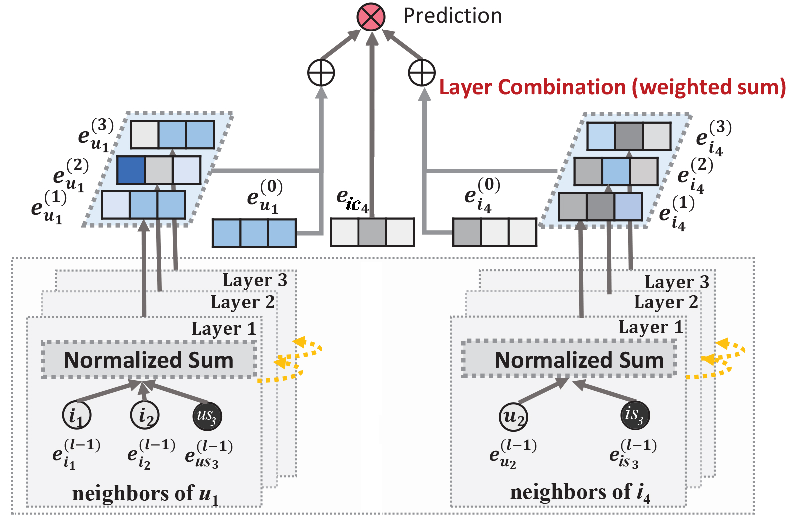
\includegraphics[width=0.48\textwidth]{figures/CSGCN.pdf}\vspace{-5pt}
%   \caption{An illustration of CSGCN-IS model architecture. User and item neighbors are illustrated as bright nodes, and side-information as dark nodes. In the layer combination, we sum over the embeddings at each layer to obtain the final representations.}\vspace{-10pt}
%   \label{fig:csgcn_is_model}
%\end{figure}
%The model itself is very similar to LightGCN.
%It is, however, important to note that the neighboring nodes for users now include side-information for users and not only items, which can be seen in each of the layers now receiving a normalized sum of both items and user side-information, rather than just the normalized sum of items.
%The same goes for the neighbors of items.

\subsection{Adjacency matrix}\label{subsec:csgcn_is_adj_mat}
As described in \Cref{sec:preliminaries}, GCNs used for CF recommendation typically employ a bipartite graph structure to represent the user-item interactions.
In CSGCN-IS the extended graph now contains users, items and edges as well as the set of user side-information nodes $US$ and the set of item side-information nodes $IS$.
This allows for the incorporation of the side-information in the model, whereas context is later included in the prediction function defined in \autoref{subsec:csgcn_is_score_prediction}.
This graph extension can be seen on \Cref{fig:quadripartite-graph}.
It should be noted that the distinct sets cannot be self-connected, and edges can only exist between adjacent sets.
Formally, we let $G$ be a graph consisting of a set of edges $E$, and vertices $V$, where $V = US \cup U \cup I \cup IS$.
$$E_{US} \subseteq \{ (x,y) | \: x \in US, \: y \in U  \}$$
$$E_U \subseteq \{ (x,y) | \: x \in U, \: y \in US \cup I \}$$
$$E_I \subseteq \{ (x,y) | \: x \in I, \: y \in U \cup IS \}$$
$$E_{IS} \subseteq \{ (x,y) | \: x \in IS, \: y \in I  \}$$
$$E = E_{US} \cup E_{U} \cup E_{I} \cup E_{IS} $$

\begin{figure}[h]
\begin{tikzpicture}[thick,
    every node/.style={draw,circle},
    inode/.style={fill=myred},
    unode/.style={fill=myblue},
    isnode/.style={fill=green},
    usnode/.style={fill=yellow},
    every fit/.style={ellipse,draw,inner sep=-2pt,text width=1.3cm},
    shorten >= 3pt,shorten <= 3pt
  ]
  
  % the vertices of US
  \begin{scope}[start chain=going below,node distance=7mm]
  \foreach \i in {us1,us2,us3}
    \node[usnode,on chain] (\i) [] {};
  \end{scope}
  
  % the vertices of U
  \begin{scope}[xshift=2cm,start chain=going below,node distance=7mm]
  \foreach \i in {u1,u2,u3}
    \node[unode,on chain] (\i) [] {};
  \end{scope}
  
  % the vertices of I
  \begin{scope}[xshift=4cm,start chain=going below,node distance=7mm]
  \foreach \i in {i1,i2,i3,i4}
    \node[inode,on chain] (\i) [] {};
  \end{scope}
  
  % the vertices of IS
  \begin{scope}[xshift=6cm,start chain=going below,node distance=7mm]
  \foreach \i in {is1,is2,is3,is4}
    \node[isnode,on chain] (\i) [] {};
  \end{scope}
  
  % the set U
  \node [myblue,fit=(u1) (u3),label=above:$U$] {};
  % the set I
  \node [myred,fit=(i1) (i4),label=above:$I$] {};
  % the set US
  \node [yellow,fit=(us1) (us3),label=above:$US$] {};
  % the set IS
  \node [green,fit=(is1) (is4),label=above:$IS$] {};
  
  % the edges
  \draw (us1) -- (u2);
  \draw (us2) -- (u1);
  \draw (us3) -- (u3);
  \draw (us3) -- (u1);
  \draw (u1) -- (i3);
  \draw (u2) -- (i2);
  \draw (u3) -- (i1);
  \draw (u2) -- (i4);
  \draw (i1) -- (is3);
  \draw (i2) -- (is1);
  \draw (i3) -- (is1);
  \draw (i4) -- (is4);
  \draw (i3) -- (is2);
\end{tikzpicture}
\caption{Example of the quadripartite graph structure used for CSGCN-IS.}
\label{fig:quadripartite-graph}
\end{figure}
The quadripartite graph can be represented as an adjacency matrix $A \in \mathbb{R}^{|U|\times|I|\times|US| \times |IS|}$.
An entry is 1 if the user has interacted with the item, if the item has the given side-information or if a user has the given side-information, and 0 if none of these are true.
$A$ consists of the rating matrix $R$ and its transpose $R^T$, as well as sub-matrices containing $US$, $IS$, and their transposes, as seen on \Cref{csgcn_is_adj_mat}.
\begin{equation}\label{csgcn_is_adj_mat}
    \begin{bmatrix}
    0 & R & US & 0\\
    R^T & 0 & 0 & IS\\
    US^T & 0 & 0 & 0 \\
    0 & IS^T & 0 & 0
    \end{bmatrix}
\end{equation}
Since there are no interactions between users and users, the first quadrant is a zero-matrix of size $$|U|\times|U|$$ where $|U|$ is the amount of users in the dataset.
This goes for all the zero matrices seen on $A$, making it mostly sparse.
Adding the side-information to the adjacency matrix allows us to express the connections between users and items and their side-information in the graph, allowing it to be used in order to gain higher-order connectivity in the convolution layers.
It is worth noting that, unlike traditional GCNs, CSGCN does not utilize self-connections since the layer combination performed after the convolution layers captures the same effect as self-connections through the 0th layer \cite{LightGCN}.
\\\\
The matrix form of CSGCN-IS is similar to the one described in \cite{LightGCN}, except for the adjacency matrix being modified as described above.
Let the embedding matrix for the 0th layer be $Emb^{(0)} \in \mathbb{R}^{(|U| + |I| + |US| + |IS|) \times K}$, where $K$ is the embeddings size, then the embedding matrix for the next layer $l+1$ can be obtained by:
\begin{equation}
    Emb^{(l+1)} = (D^{-\frac{1}{2}}AD^{-\frac{1}{2}})Emb^{(l)}
\end{equation}
where $l$ is the current layer and $D$ is a $(|U| + |I| + |US| + |IS| \times (|U| + |I| + |US| + |IS|)$ degree matrix. 
The final embedding matrix after $L$ layers is defined as:
\begin{equation}
    Emb = \frac{1}{0 +1}Emb^{(0)} + \frac{1}{1 +1}Emb^{(1)} + \cdots + \frac{1}{l +1}Emb^{(L)}
\end{equation}

\subsection{Convolution layers}\label{subsec:csgcn_is_conv_layer}
A major part of the model is the convolution layer where the user and item embeddings are being propagated with information about their neighbor nodes' representations by using an aggregation function, which in this case is a normalized sum.
Neighbor nodes for users are item nodes and user side-information nodes, and for items the neighbors are user nodes and item side-information nodes, which can be seen on \Cref{fig:quadripartite-graph}.
For each additional layer, information is passed from nodes that are further away from a central node, illustrated on \Cref{fig:aggregation-for-layers}.
\begin{figure}[h]
    \centering
    \tikzset{every picture/.style={line width=0.75pt}} %set default line width to 0.75pt        
    
    \begin{tikzpicture}[x=0.5pt,y=0.5pt,yscale=-1,xscale=1]
    %uncomment if require: \path (0,300); %set diagram left start at 0, and has height of 300
    
    %Flowchart: Connector [id:dp27406580802635316] 
    \draw   (290.75,139) .. controls (290.75,126.85) and (300.6,117) .. (312.75,117) .. controls (324.9,117) and (334.75,126.85) .. (334.75,139) .. controls (334.75,151.15) and (324.9,161) .. (312.75,161) .. controls (300.6,161) and (290.75,151.15) .. (290.75,139) -- cycle ;
    %Flowchart: Connector [id:dp597318920352127] 
    \draw   (289,81) .. controls (289,68.85) and (298.85,59) .. (311,59) .. controls (323.15,59) and (333,68.85) .. (333,81) .. controls (333,93.15) and (323.15,103) .. (311,103) .. controls (298.85,103) and (289,93.15) .. (289,81) -- cycle ;
    %Flowchart: Connector [id:dp057928841134587516] 
    \draw   (350,143) .. controls (350,130.85) and (359.85,121) .. (372,121) .. controls (384.15,121) and (394,130.85) .. (394,143) .. controls (394,155.15) and (384.15,165) .. (372,165) .. controls (359.85,165) and (350,155.15) .. (350,143) -- cycle ;
    %Flowchart: Connector [id:dp11200641374570286] 
    \draw   (289,197) .. controls (289,184.85) and (298.85,175) .. (311,175) .. controls (323.15,175) and (333,184.85) .. (333,197) .. controls (333,209.15) and (323.15,219) .. (311,219) .. controls (298.85,219) and (289,209.15) .. (289,197) -- cycle ;
    %Flowchart: Connector [id:dp5153973147602738] 
    \draw   (231,137) .. controls (231,124.85) and (240.85,115) .. (253,115) .. controls (265.15,115) and (275,124.85) .. (275,137) .. controls (275,149.15) and (265.15,159) .. (253,159) .. controls (240.85,159) and (231,149.15) .. (231,137) -- cycle ;
    %Flowchart: Connector [id:dp6230129861696904] 
    \draw   (197,59) .. controls (197,46.85) and (206.85,37) .. (219,37) .. controls (231.15,37) and (241,46.85) .. (241,59) .. controls (241,71.15) and (231.15,81) .. (219,81) .. controls (206.85,81) and (197,71.15) .. (197,59) -- cycle ;
    %Flowchart: Connector [id:dp11627558541491778] 
    \draw   (181,213) .. controls (181,200.85) and (190.85,191) .. (203,191) .. controls (215.15,191) and (225,200.85) .. (225,213) .. controls (225,225.15) and (215.15,235) .. (203,235) .. controls (190.85,235) and (181,225.15) .. (181,213) -- cycle ;
    %Flowchart: Connector [id:dp012014051199046416] 
    \draw   (374,61) .. controls (374,48.85) and (383.85,39) .. (396,39) .. controls (408.15,39) and (418,48.85) .. (418,61) .. controls (418,73.15) and (408.15,83) .. (396,83) .. controls (383.85,83) and (374,73.15) .. (374,61) -- cycle ;
    %Flowchart: Connector [id:dp025105219979997373] 
    \draw   (375,220) .. controls (375,207.85) and (384.85,198) .. (397,198) .. controls (409.15,198) and (419,207.85) .. (419,220) .. controls (419,232.15) and (409.15,242) .. (397,242) .. controls (384.85,242) and (375,232.15) .. (375,220) -- cycle ;
    %Flowchart: Connector [id:dp28306483017107376] 
    \draw  [color={rgb, 255:red, 255; green, 0; blue, 0 }  ,draw opacity=1 ][dash pattern={on 4.5pt off 4.5pt}] (282,139) .. controls (282,121.88) and (295.77,108) .. (312.75,108) .. controls (329.73,108) and (343.5,121.88) .. (343.5,139) .. controls (343.5,156.12) and (329.73,170) .. (312.75,170) .. controls (295.77,170) and (282,156.12) .. (282,139) -- cycle ;
    %Flowchart: Connector [id:dp22791557868185153] 
    \draw  [color={rgb, 255:red, 255; green, 0; blue, 0 }  ,draw opacity=1 ][dash pattern={on 4.5pt off 4.5pt}] (223.75,139) .. controls (223.75,90) and (263.15,50.28) .. (311.75,50.28) .. controls (360.35,50.28) and (399.75,90) .. (399.75,139) .. controls (399.75,188) and (360.35,227.72) .. (311.75,227.72) .. controls (263.15,227.72) and (223.75,188) .. (223.75,139) -- cycle ;
    %Flowchart: Connector [id:dp946514520124221] 
    \draw  [color={rgb, 255:red, 255; green, 0; blue, 0 }  ,draw opacity=1 ][dash pattern={on 4.5pt off 4.5pt}] (147.5,142.5) .. controls (147.5,64.9) and (219.13,2) .. (307.5,2) .. controls (395.87,2) and (467.5,64.9) .. (467.5,142.5) .. controls (467.5,220.1) and (395.87,283) .. (307.5,283) .. controls (219.13,283) and (147.5,220.1) .. (147.5,142.5) -- cycle ;
    %Straight Lines [id:da566741285857424] 
    \draw    (235.5,72) -- (288.5,74) ;
    %Straight Lines [id:da31194843739323463] 
    \draw    (228.5,78) -- (238.5,121) ;
    %Straight Lines [id:da32353885946741523] 
    \draw    (240.5,156) -- (212.5,193) ;
    %Straight Lines [id:da5053069271391968] 
    \draw    (311,103) -- (312.75,117) ;
    %Straight Lines [id:da723620476456976] 
    \draw    (290.75,139) -- (275,137) ;
    %Straight Lines [id:da14267027138513144] 
    \draw    (312.75,161) -- (311,175) ;
    %Straight Lines [id:da6090096595211273] 
    \draw    (334.75,139) -- (350,143) ;
    %Straight Lines [id:da11771537978983193] 
    \draw    (396,83) -- (372,121) ;
    %Straight Lines [id:da45445879447578685] 
    \draw    (332.5,206) -- (375,220) ;
    
    % Text Node
    \draw (305,129) node [anchor=north west][inner sep=0.75pt]   [align=left] {U};
    % Text Node
    \draw (298,70) node [anchor=north west][inner sep=0.75pt]   [align=left] {US};
    % Text Node
    \draw (364,132) node [anchor=north west][inner sep=0.75pt]   [align=left] {I};
    % Text Node
    \draw (305,186) node [anchor=north west][inner sep=0.75pt]   [align=left] {I};
    % Text Node
    \draw (240,126) node [anchor=north west][inner sep=0.75pt]   [align=left] {US};
    % Text Node
    \draw (211,48) node [anchor=north west][inner sep=0.75pt]   [align=left] {U};
    % Text Node
    \draw (195,202) node [anchor=north west][inner sep=0.75pt]   [align=left] {U};
    % Text Node
    \draw (387,50) node [anchor=north west][inner sep=0.75pt]   [align=left] {IS};
    % Text Node
    \draw (389,209) node [anchor=north west][inner sep=0.75pt]   [align=left] {IS};
    % Text Node
    \draw (332,97) node [anchor=north west][inner sep=0.75pt]   [align=left] {l=0};
    % Text Node
    \draw (396,94) node [anchor=north west][inner sep=0.75pt]   [align=left] {l=1};
    % Text Node
    \draw (463,89) node [anchor=north west][inner sep=0.75pt]   [align=left] {l=2};
    
    
    \end{tikzpicture}
    
    \caption{Information aggregated through layers.}
    \label{fig:aggregation-for-layers}
    \end{figure}
The representations at each of the layers are aggregated into a final representation after $l$ layers.
From these final representations, a score prediction can be calculated between an item, user and a context which is further described in \Cref{subsec:csgcn_is_score_prediction}.
The inputs to the layer is the adjacency matrix previously described.

\begin{equation}\label{eq:csgcn_is_gc_layer_item}
    e_{i}^{(l+1)}=\sum_{in\in \mathcal{N}_{i}}\frac{1}{\sqrt{|\mathcal{N}_{i}|} \sqrt{|\mathcal{N}_{in}|}}e_{in}^{(l)}
\end{equation}

\begin{equation}\label{eq:csgcn_is_gc_layer_user}
     e_{u}^{(l+1)}=\sum_{un\in \mathcal{N}_{u}}\frac{1}{\sqrt{|\mathcal{N}_{un}|} \sqrt{|\mathcal{N}_{u}|}}e_{un}^{(l)}
\end{equation}

In \Cref{eq:csgcn_is_gc_layer_item,eq:csgcn_is_gc_layer_user} the convolution operation is shown for respectively item and user embeddings, where $\mathcal{N}_{u}$ are the neighbor nodes for user $u$, where $\mathcal{N}_{u} \subseteq US \cup I$, and $\mathcal{N}_{i}$ are the neighbor nodes for item $i$ where $\mathcal{N}_{i} \subseteq IS \cup U$.\\
A user neighbor node is denoted as $un \in \mathcal{N}_{u}$, and for item neighbors as $in \in \mathcal{N}_{i}$.
$N_{un}$ denotes the set of neighbors for the neighbor $un$ of node $u$, and $N_{in}$ denotes the set of neighbors for the neighbor $in$ of node $i$.\\
This means that when neighbor nodes' representations are being propagated, the normalization is done with both the number of neighbors for the central node and the number of neighbors of the neighbor node that is currently having its representation propagated.
\\\\
The convolution layer propagates information to user and item nodes' representations by summing the normalized representations of the neighbor nodes.
All types of nodes are being propagated with information about their neighbors, but since only the user and item nodes' representations are being used in the prediction function for our model, their representations are the only ones that are output from the convolution layer.
% The argument for not also outputting side-information nodes and using these in the prediction function is that, through the convolution, the information from these nodes is integrated into the representations of user and item nodes.

\subsection{Score prediction}\label{subsec:csgcn_is_score_prediction}
To include context in the score prediction, we propose to model each pair of items and context values as learnable embeddings $e_{ic}$.
The use of $e_{ic}$ is heavily inspired by Ricci and Baltrunas' item splitting approach \cite{baltrunasitemsplitting}, where a context weight for each item in each context is calculated.
This means that for the set of items $I$ and the set of possible context values $C$, there are $|I| \times |C|$ embeddings of item and context value combinations $e_{ic}$.
The objective is to calculate a score between a user and an item in a given context $C'$.
The different $e_{ic}$'s of a given item $i$ and context $C'$ are added to the item to signify its popularity in the given context.
After the addition of the $e_{ic}$'s to the item embedding $e_i$, the cosine similarity scores of the user embedding $e_u$ and the item-context additions are calculated and summed together to produce a score: 
\begin{equation}
  \hat{y}_{uic} = \sum_{c \in C'} e_u^T(e_i+e_{ic})
\end{equation}
As shown, the context embeddings are not part of the convolution layer but are only used in the score prediction, meaning that they are learned directly through their appearance in the score prediction function.


\subsection{Training}\label{subsec:csgcn_is_training}
For the top-$k$ recommendation task, we utilize negative sampling and Bayesian Pairwise Ranking (BPR) loss \cite{BPR} as the training function, shown in \autoref{eq:loss-func}.
\begin{equation}\label{eq:loss-func}
    Loss = \sum_{(u,i,j,C') \in D_T} \sigma(-(\hat{y}_{(u,i,C')} - \hat{y}_{(u,j,C')})) + \lambda_\Theta ||\Theta||^2
\end{equation}
where $\Theta$ denotes the trainable model parameters, which in this case are the 0th layer embeddings for items ($e_{i}^{(0)}$) and users ($e_{u}^{(0)}$), as well as the embeddings for side-information ($e_{us}$ and $e_{is}$) and item-context embeddings ($e_{ic}$).
$\lambda$ denotes the regularization coefficient, and $\sigma(\cdot)$ denotes the non-linear activation function, in this case, the softplus function.\\
The regularization term $\lambda_\Theta ||\Theta||^2$ is included to prevent overfitting.
$D_T = \{(u,i,j,C'') | i \in I_{(u,C')} \wedge  j \in I \setminus I_{(u,C')}\}$ denotes the dataset of training tuples, where $I_{(u,C')}$ is the set of observed items that user $u$ has interacted with in context $C'$.
$\hat{y}$ is a score prediction for respectively a positive interaction $(u,i,C')$ between a user $u$ and an item $i$ in context $C'$, and a negative interaction $(u,j,C')$ for the same user in the same context, where $j$ is an item the user has not interacted with.\\
The positive interaction is an observed interaction between a user and an item, which can be found in the training set.
We randomly select an item that the same user has not interacted with in this given context as a negative sample, with the assumption that an unobserved interaction is equal to a negative interaction when working with implicit data.\\
Using negative sampling for calculating loss is biased \cite{nonsampling,NegativeSampling}, and sensitive to the number of negative samples \cite{NCF}.
Fluctuations in the sampled negative item can cause difficulties in converging, and even sampling more negative items can increase performance.\\
Chen et al. \cite{nonsampling} propose to learn FM models without negative sampling to improve ranking performance for context-aware recommendation, and increase stability due to considering all samples in each parameter update.
However, using negative sampling can be necessary since using non-sampling not only requires the method to look at each observed interaction from the dataset, but also to consider each non-observed interaction as a negative data point.
Because of this consideration, CSGCN-IS uses negative sampling for training, and, due to employing BPR loss, only one negative sample is used.
\\\\
The model parameters are updated by optimizing the BPR loss function in \Cref{eq:loss-func}.
For a specific model parameter, this is done by calculating the gradient of the loss function at each iteration with respect to the model parameter, and then updating the parameter according to the gradient by a step size defined through the learning rate.
The gradient is a vector of partial derivatives which defines the slope of the function, where a partial derivative of a function with multiple variables is the derivate with respect to a single variable with the remaining variables held constant.
The derivative defines how the output of the function changes based on changes in the input.
The model parameters can then be updated in the negative direction of the slope of the function, the gradient, based on the learning rate in order to approach a local minima. 
In our implementation, the loss function is optimized using the \textit{Adam Optimizer} \cite{AdamOptimizer}, based on empirical testing.
Optimizer functions are an essential part of machine learning, since they are used to tune the parameters of the neural network to minimize the loss function.
The chosen optimizer can impact the training speed and final performance of the model.
However, there is no theory that explains how to decide which optimizer to use \cite{EmpiricalOptimizers}.
Unlike simpler optimizers that maintain a single learning rate throughout training, such as stochastic gradient descent, Adam utilizes an adaptive per-parameter learning rate by estimating the mean and the variance of the gradient and the squared gradient \cite{AdamOptimizer}.
Additionally, Adam is reliable for calculating gradients in sparse situations, which is an important property for RS, since they often deal with sparse data.

\section{CSGCN-ADJ}\label{sec:csgcn_adj}
This section describes the second proposed model, CSGCN with Context in Adjacency Matrix (CSGCN-ADJ).

\subsection{Model intuition}\label{subsec:csgcn_adj_intuition}
With the second proposed model, context is included in the convolution by adding context nodes to the graph, which will be used to represent interactions between users and items in a given context as a tuple $(u,i,C')$, implying that a user $u$ has interacted with item $i$ in context $C'$.
The adjacency matrix will now include interactions, which contexts the users have interacted in, and the contexts in which items have been interacted with.
This approach is unable to capture which specific context a given interaction occurred in.
It only captures whether or not the user or item has had an interaction in the given context.
This differs from \textit{CSGCN-IS} since we now model context in a similar fashion to side-information, where each context value has a single embedding instead of having an embedding for each context value and item pair.
The intuition is that since context is now modeled similarly to side-information by the addition of nodes, it makes sense to include it in the convolution.
By including nodes for the contexts in the convolution, their representations are propagated with information about their neighbors, this being items and users that have interacted in that context, using a normalized sum aggregation.
This means that with higher-order connectivity, items and users are propagated with information about other users and items that have interacted in the same contexts.
Even though the intuition changes, the model architecture is almost the same as defined in \Cref{subsec:csgcn_is_model_architecture}.
The difference is that the input graph to the convolution layers now includes context nodes, meaning they are also a part of the neighborhood aggregations.

\subsection{Adjacency matrix}\label{subsec:csgcn_adj_adj_mat}
Compared to CSGCN-IS, context is now included in the graph as nodes and therefore also included in the adjacency matrix.
The graph is similar to the one in \Cref{fig:quadripartite-graph}, but context nodes are inserted between the sets of item and user nodes, and edges connect the nodes that have interacted in the context.
This results in the sets of edges $E_U$ and $E_I$ being updated to:
$$E_U \subseteq \{ (x,y) | \: x \in U, \: y \in US \cup I \cup C \}$$
$$E_I \subseteq \{ (x,y) | \: x \in I, \: y \in U \cup IS \cup C \}$$
A new set of edges is also introduced for the context value nodes in $C$:
$$E_C \subseteq \{ (x,y) | \: x \in C, \: y \in U \cup I \}$$
For the convolution, we want to preserve the context's initial embeddings from the first layer through to the last layer, since we found that this gave slightly better performance compared to also propagating information about neighbors to the context embeddings.
Therefore, the transposed matrices of $UC$ and $IC$ are not inserted into the adjacency matrix.
Instead, we add the identity matrix $I$ to the last quadrant such that the context embeddings are only propagated with information about themselves in each convolution.
The matrix is seen in \Cref{csgcn_adj_adj_mat}.
\begin{equation}\label{csgcn_adj_adj_mat}
    \begin{bmatrix}
    0 & R & US & 0 & UC\\
    R^T & 0 & 0 & IS & IC\\
    US^T & 0 & 0 & 0 & 0\\
    0 & IS^T & 0 & 0 & 0 \\
    0 & 0 & 0 & 0 & I
    \end{bmatrix}
\end{equation}
Let the embedding matrix for the 0th layer be $Emb^{(0)} \in \mathbb{R}^{(|U| + |I| + |US| + |IS| + |C|) \times K}$, where $K$ is the embedding size and $C$ is the set of possible context values.
The embedding matrix for the next layer after $l$ for CSGCN-ADJ is obtained by:
\begin{equation}
    Emb^{(l+1)} = (D^{-\frac{1}{2}}A)Emb^{(l)}
\end{equation}
where $l$ is the current layer and $D$ is a $(|U| + |I| + |US| + |IS| + |C|) \times (|U| + |I| + |US| + |IS|+ |C|)$ degree matrix. 
We see that for this model, we only normalize on a row-level by multiplying by $D^{-\frac{1}{2}}$ on the left side of the adjacency matrix.
This approach is inspired by a combination of the random walk Laplacian $D^{-1}A$ and the symmetrical normalized Laplacian $D^{-\frac{1}{2}}AD^{-\frac{1}{2}}$ used in CSGCN-IS.
We found that for this model, it gave slightly better performance compared to these regular normalization methods, as evidenced by the results seen on \Cref{fig:normalization_graph}.
While this graph only shows the results for NDCG@20 on the Yelp-NC dataset, the trend is consistent across datasets and metrics.

\begin{figure}
    \begin{tikzpicture}
        \begin{axis}[
            xlabel=Epoch,
            ylabel=NDCG@20,
            height=8cm,
            width=7cm,
            grid=major,
            legend style={at={(0.5,-0.20)},
        anchor=north,legend columns=2}]

        \addplot plot coordinates{
            (20,0.05145)
            (40,0.0642)
            (60,0.06552)
            (80,0.06201)
            (100,0.06508)
            (120,0.07168)
            (140,0.07256)
            (160,0.073)
            (180,0.06992)
            (200,0.07344)
        };

        \addplot plot coordinates{
            (20,9.0629e-3)
            (40,8.9258e-3)
            (60,9.0337e-3)
            (80,8.3179e-3)
            (100,7.771e-3)
            (120,7.8698e-3)
            (140,8.4826e-3)
            (160,9.2474e-3)
            (180,9.5092e-3)
            (200,0.0106)
        };

        \addplot plot coordinates{
            (20,8.7e-3)
            (40,8.8121e-3)
            (60,8.9353e-3)
            (80,8.6377e-3)
            (100,8.065e-3)
            (120,7.7449e-3)
            (140,7.9213e-3)
            (160,8.1782e-3)
            (180,8.9256e-3)
            (200,8.9743e-3)
        };

        \legend{$D^{-\frac{1}{2}}$,$D^{-1}A$,$D^{-\frac{1}{2}}AD^{-\frac{1}{2}}$}
        \end{axis}
    \end{tikzpicture}
    \caption{Effect of various normalizations for CSGCN-ADJ on the Yelp-NC dataset for HR@20.}
    \label{fig:normalization_graph}
\end{figure}
The final embedding matrix after $l$ layers is obtained in the same way as CSGCN-IS where we take the mean of the nodes' representations at each layer.

\subsection{Convolution layers}\label{subsec:csgcn_adj_conv_layer}
For the graph convolution layer of CSGCN-ADJ, the context is incorporated into the aggregation of neighbors seen in \Cref{eq:csgcn_adj_gc_layer_item,eq:csgcn_adj_gc_layer_user}
\begin{equation}\label{eq:csgcn_adj_gc_layer_item}
    e_{i}^{(l+1)}=\sum_{in\in \mathcal{N}_{i}}\frac{1}{\sqrt{|\mathcal{N}_{i}|} }e_{in}^{(l)}
\end{equation}

\begin{equation}\label{eq:csgcn_adj_gc_layer_user}
     e_{u}^{(l+1)}=\sum_{un\in \mathcal{N}_{u}}\frac{1}{ \sqrt{|\mathcal{N}_{u}|}}e_{un}^{(l)}
\end{equation}
With this convolution, only the number of neighbors of the node that is being propagated information to is used for normalization.
As a result of context being added as nodes in the graph for CSGCN-ADJ, $\mathcal{N}_{u}$ also contains the contexts that user $u$ has interacted in and $\mathcal{N}_{i}$ also contains the contexts that item $i$ has interacted in.
Because the identity matrix was added to the adjacency matrix under the context columns, the context embeddings retain their initial values throughout the convolution layer.

\subsection{Score prediction and training}\label{subsec:csgcn_adj_score_pred}
For the score prediction of CSGCN-ADJ, we draw inspiration from factorization machines and use an FM-like predictor function that considers pair-wise interactions between users, items and context values to provide a recommendation.
To do this, we use the prediction function defined in \Cref{eq:csgcn_adj_scorepred}:
\begin{equation}\label{eq:csgcn_adj_scorepred}
    \hat{y}_{uic} = e_u^Te_i + \sum_{c \in C'}e_u^Te_{c} + \sum_{c \in C'}e_i^Te_{c}
\end{equation}
Where $e_{c}$ is the embedding representation of the context value $c$, $e_i$ is the embedding of the item $i$ and $e_u$ is the embedding of the user $u$.
In this predictor function, we calculate the pairwise interaction between each of the embeddings.
The self-interactions are not calculated since they do not contribute to the score prediction.
The embeddings used for items and users are the ones output by the convolution layer while the context embeddings are the initial values before convolution, since they are only propagated with information about themselves.
\\
Training of CSGCN-ADJ is similar to that of CSGCN-IS, using the same loss function and the Adam optimizer.

\section{Experiments}\label{sec:experiments}
Experiments are conducted in this section in order to answer the following research questions:
\begin{itemize}
    \item \textbf{RQ1}: How do the CSGCN models compare to state-of-the-art methods for the task of context-aware list prediction?
    \item \textbf{RQ2}: Can the CSGCN models be used to make non-context specific recommendations?
    \item \textbf{RQ3}: Does side-information improve results for context-aware recommendations?
\end{itemize}
The section details the experimental settings used, the datasets, the methods, and the metrics employed for comparison.

\subsection{Datasets}\label{subsec:experimental-settings}
To test the models on datasets with varying sizes and density, the following datasets were chosen:\\

\begin{adjustwidth}{-2.5 cm}{-2.5 cm}\centering
\begin{threeparttable}[]
\scriptsize
\begin{tabular}{lcccccc}\toprule
\textbf{Dataset} &\textbf{User \#} &\textbf{Item \#} &\textbf{Interaction \#} &\textbf{Context \#} &\textbf{Sideinfo \#} \\\cmidrule{1-6}
ML1m &6,040 &3,377 &999,416 &2 &4 \\\cmidrule{1-6}
%ML100k &943 &1,682 &100,000 &4 &4 \\\cmidrule{1-6}
Frappe &546 & 821 &85,541 &6 &1 \\\cmidrule{1-6}
Yelp-NC &2,274 &2,140 &130,627 &1 &3 \\\cmidrule{1-6}
Yelp-ON &5,185 &5,566 &332,291 &1 &3 \\\midrule
\bottomrule
\end{tabular}
\caption{Statistics of the datasets.}\label{tab:datasetstats}
\end{threeparttable}
\end{adjustwidth}

\subsubsection*{MovieLens 1M (ML1M)}
ML1M is a dataset \cite{ml1m} with 1 million interactions between 6,040 users and 3,377 movies.\\
We use the following side-information for users:
\begin{itemize}
    \item Age
    \item Gender
    \item Occupation
\end{itemize}
Side-information for items is \textit{genre}, which specifies that an item has one or more of the 18 genres available in the dataset.
For contextual information, the MovieLens dataset provides a timestamp for when the interaction took place.

\subsubsection*{Frappe}
The Frappe dataset \cite{baltrunasfrappe} contains information about how users have interacted with applications on their smartphones.
The only available side-information is for items, indicating whether the application is free or not.
However, it contains the following contexts:
\begin{itemize}
    \item City
    \item Country
    \item Weekday
    \item Time of day
    \item Whether it is weekend or not
    \item Weather
\end{itemize}

\subsubsection*{Yelp-NC and Yelp-ON}
The two Yelp datasets, Yelp-NC and Yelp-ON, are subsets of the public Yelp dataset \cite{yelp}, where we take the subset of items located in respectively North Carolina (NC) and Ontario (ON).
Both Yelp datasets have been pruned such that it includes only users with at least 10 interactions, to facilitate generating a stratified data split where each user in the test set is also in the training set.\\
We use the following side-information about users for both datasets:
\begin{itemize}
    \item Yelping since (Year)
    \item Number of fans
    \item Average stars
\end{itemize}
The side-information about items is a dimension specifying the categories that an item belongs to.
For the Yelp-NC dataset, this is one or more of 80 different categories, and 75 categories for Yelp-ON.\\
The contextual information is a timestamp.

\subsection{Context dimension selection}
Since most of the datasets include a timestamp as contextual information, we discretize these into the following context dimensions:
\begin{itemize}
    \item Month
    \item Day of week
    \item Hour
    \item Time of day
\end{itemize}
Where time of day is a further discretization of the hour dimension, split into 5 intervals:
\begin{itemize}
    \item Night (0 to 4)
    \item Early morning (4 to 8)
    \item Late morning (8 to 12)
    \item Evening (12 to 16)
    \item Afternoon (16 to 20)
    \item Late night (20 to 24)
\end{itemize}
For the Frappe dataset, we instead make use of the 6 contextual values available in the dataset.
\\\\
For the side-information, we use the dimensions mentioned in \Cref{subsec:experimental-settings} for both users and items with some discretization.
The Yelp datasets provide a "yelping since" dimension, which is a timestamp for the creation of the user.
This is discretized to include only the year that the user has been created.
\\
Additionally, the dimension "fans" is discretized into four groups:
\begin{itemize}
    \item $< 50$ fans
    \item $50 - 100$ fans
    \item $100-500$ fans
    \item $> 500$ fans
\end{itemize}

\subsection{Compared methods}
In the experiments, the CSGCN models are compared against the following methods for context-specific recommendations:
\begin{itemize}
    \item Factorization Machine (FM)\cite{fmrendle}
    \item Convolutional Factorization Machine (CFM) \cite{CFM}
    \item Neural Factorization Machine (NFM) \cite{NeuralFM}
    % \item Top Pop
    % \item CAMF \cite{CAMF}
\end{itemize}
CFM uses a combination of a CNN and an FM, which is similar to our method in that it is capable of producing a context-aware top-$k$ recommendation list.
It is included since it is an alternative way to handle contextual information in CNNs.
We also compare against NFM, which uses a multi-layer perceptron (MLP) on top of the factorization machine to learn higher-order interaction signals.
\\\\
To compare the performance of the models in a non-context specific setting, we compare against the following methods:
\begin{itemize}
    \item Neural Graph Collaborative Filtering (NGCF) \cite{NGCF}
    \item Light Graph Convolutional Network (LightGCN) \cite{LightGCN}
    \item Knowledge Graph Attention Network (KGAT) \cite{KGAT}
    \item Bayesian Personalized Ranking (BPR) \cite{BPR}
    \item Top Pop
    %\item Factorization Machine \cite{fmrendle}
\end{itemize}
Both the CSGCN models and LightGCN extend the codebase of NGCF, so they are included in the comparison to show that adding side-information contextual information hopefully improves the accuracy of these methods.\\
KGAT is a state-of-the-art graph-based method that utilizes side-info in the form of a knowledge graph.
BPR utilizes implicit feedback to generate a personalized top-$k$ list of items using the proposed BPR-optimizer to train the model, providing a simpler method for comparison.
Finally, a we include a simple baseline, Top Pop, which simply recommends the $k$ most popular items for all users.

\subsection{Parameter settings}
To fairly compare the performance of the models, we train all of them by optimizing the BPR loss with Adam.
The learning rate is either set to the value presented in the respective papers, or searched between $[0.1, 0.01, 0.001, 0.0001]$ if a default is not available.
The batch size is set as 1024 for all datasets except Frappe, where it is set to 512 due to its size.
The embedding size is set to 64, and for the models using regularization terms, this is searched between $[0.01, 0.001, 0.0001]$ if a default value is not provided.
For CFM and NFM we follow the approach presented in the original papers and feed them with weights from a pretrained FM model which has run for 500 epochs with the settings presented in the CFM paper.
All methods are run for a max of 1000 epochs with an early stopping mechanism triggered when the HR@20 or Recall@20 has not improved for 5 evaluations (100 consecutive steps), except for CFM which is run for 300 epochs based on the default values.


\subsection{Evaluating the models}\label{subsec:evalandmetrics}
The objectives of the models in the experiments are to produce top-$k$ lists of items for a user. 
Different methods for evaluating the performances of the models were considered, specifically the fold-out and leave-one-out methods.
These methods interact with the context in different ways.
For the fold-out method, the datasets are split into a training set and a test set, where the model is trained on the training set and evaluated on the test set. 
This split is generated such that each user in the test set is also found in the training set.
Using this stratified split method, we decided to use a split of 80\% training and 20\% test split.
Because of this split, a single user can have multiple ground truth entries across multiple contexts.\\
A problem to consider with fold-out for context-aware evaluation is that when the context is part of the input to the model, a score must be calculated for each combination of item and context due to the multiple ground truth contexts, which can be computationally expensive.
A single context cannot be guaranteed for the user for all ground truths, and thus every context needs to be evaluated.
\\\\
For the leave-one-out method, the newest interaction for each user is removed from the training set and used as the test set, as per \cite{CFM, BPR}.
This means that when a top-$k$ list is produced for a user, only a single item amongst the recommended items can be relevant, and thus there is only one context within which the ground truth had occurred.
This approach is largely inspired by sequential recommendation systems, where you leave out the newest interaction from each user and try to predict the next item in the sequence based on the sequence of the previous interactions by the user \cite{aggarwal2016recommender}.\\
This approach limits the number of different metrics that can be used for this type of evaluation method.
\\\\
For comparisons we conduct an experiment using fold-out for models that produce a top-$k$ recommendation list and conduct a separate leave-one-out evaluation for models that produce a context-aware top-$k$ recommendation list. 
The metrics used for the fold-out evaluation are Precision, Recall, and Normalized Discounted Cumulative Gain (NDCG), while the leave-one-out experiments report Hit Rate (HR) and Mean Reciprocal Rank (MRR).

\subsubsection*{Evaluation metrics explained}
The top-$k$ recommendation problem is the task of recommending a list $L(u)$ to an active user $u$ containing $k$ items.
Evaluating the quality of a method can be done by splitting the set of items $I$ into a training set $I_{train}$ and a test set $I_{test}$ for each user.
\\
Let $T(u)$ be the the set of items that the user has interacted with in the test set.
Precision can be calculated according to \Cref{eqn:precision}, and recall according to \Cref{eqn:recall}.
Precision defines the proportion of relevant items among the predicted items, while recall is the proportion of items that were correctly predicted according to the ground truth.
\begin{equation}
    \label{eqn:precision}
    Precision@N(L) = \frac{1}{|U|} \sum\limits_{u \in U}\frac{|L(u) \cap T(u)|}{|L(u)|}
\end{equation}
\begin{equation}
    \label{eqn:recall}
    Recall@N(L) = \frac{1}{|U|} \sum\limits_{u \in U} \frac{|L(u) \cap T(u)|}{|T(u)|}
\end{equation}
Another metric to be used is NDCG \cite{dcgpaper}.
Assuming each user $u$ has a gain $g_{ui}$ from being recommended item $i$, then the average DCG for a list of $J$ items is defined in \Cref{eqn:dcg}, where $i_j$ is the item at position $j$ in the list, and the logarithm base $b$ is $2$ to ensure all positions are discounted.
This metric rewards lists that frontload relevant items.
\begin{equation}
    \label{eqn:dcg}
    DCG@N = \frac{1}{|U|} \sum\limits_{u=1}^{|U|} \sum\limits_{j = 1}^{|J|} \frac{g_{ui_j}}{log_b (j+1)}
\end{equation}
NDCG is defined in \Cref{eqn:ndcg}, where $iDCG$ is the ideal DCG, which is defined by sorting the recommended items such that the relevant items appear at the start of the list, resulting in the largest possible DCG value.
\begin{equation}
    \label{eqn:ndcg}
    NDCG@N = \frac{DCG}{iDCG}
\end{equation}
MRR \cite{MRR} is employed for the leave-one-out evaluation, defined in \Cref{eqn:mrr}.
For each user $u$ in $U$, MRR is calculated by finding the rank $r_u$ of the first relevant recommendation for each list, and then taking the mean of these ranks.
\begin{equation}
    \label{eqn:mrr}
    MRR@N = \frac{1}{|U|} \sum\limits_{u \in U}\frac{1}{r_u}
\end{equation}
The final metric used is HR.
If a relevant item for a user appears in the top-$k$ list, the $HR(u)$ for that user is $1$, otherwise it is $0$.
The final HR score is then calculated by taking the mean of all users' individual HR scores, as seen in \Cref{eqn:hr}.
\begin{equation}
    \label{eqn:hr}
    HR@N = \frac{1}{|U|} \sum\limits_{u \in U}HR(u)
\end{equation}

\subsection{Performance Comparison (RQ1)}\label{subsec:rq1}
For the first research question we want to examine how the CSGCN models compare to state-of-the-art methods within context-aware list prediction.
To investigate this, the leave-one-out method presented in \Cref{subsec:evalandmetrics} is used, such that a single interaction is left out for each user, and a list is produced based on the context that this interaction took place in.

\begin{table*}[]
\centering
\resizebox{\textwidth}{!}{%
\begin{tabular}{c|l|cccc|cc}
Dataset & Metric & FM & \multicolumn{1}{c}{NFM} & \multicolumn{1}{c}{CFM} & \multicolumn{1}{c|}{CSGCN-IS} & \multicolumn{1}{c}{CSGCN-ADJ} & \multicolumn{1}{c|}{Impr.} \\ \hline
\multirow{4}{*}{YelpNC} & HR@20  & 0.0075  & 0.0142  & 0.0070 & 0.0625 & 0.0761  &  \\
                        & HR@50  & 0.0198  & 0.0240  & 0.0163 & 0.1143 & 0.1464  &  \\
                        & MRR@20 & 0.0022  & 0.0030  & 0.0037 & 0.0127 & 0.0158  &  \\
                        & MRR@50 & 0.0025  & 0.0033  & 0.0040 & 0.0143 & 0.0179  &  \\ \hline
\multirow{4}{*}{Frappe} & HR@20  & 0.6590  & 0.3516  & 0.3242 & 0.0458 & 0.0604  &  \\
                        & HR@50  & 0.8004  & 0.4945  & 0.4560 & 0.1062 & 0.1245  &  \\
                        & MRR@20 & 0.2895  & 0.1117  & 0.1032 & 0.0128 & 0.0184  &  \\
                        & MRR@50 & 0.2942  & 0.1166  & 0.1074 & 0.0146 & 0.0204  &  \\ \hline
\multirow{4}{*}{Yelp-ON} & HR@20  & 0.0083  & 0.0085  & 0.0073 & 0.0399 & 0.0534  &  \\
                        & HR@50  & 0.0133  & 0.0152  & 0.0133 & 0.0714 & 0.0997  &  \\
                        & MRR@20 & 0.0019  & 0.0021  & 0.0019 & 0.0091 & 0.0123  &  \\
                        & MRR@50 & 0.0020  & 0.0023  & 0.0021 & 0.0101 & 0.0137  &  \\ \hline
\multirow{4}{*}{ML1M}   & HR@20  & 0.0874  & 0.0937  &        & 0.1402 & 0.1652  &  \\
                        & HR@50  & 0.1856  & 0.2005  &        & 0.2603 & 0.2982  &  \\
                        & MRR@20 & 0.0199  & 0.0209  &        & 0.0336 & 0.0372  &  \\
                        & MRR@50 & 0.0229  & 0.0242  &        & 0.0373 & 0.0413  & 
\end{tabular}%
}
\caption{Results for context-specific recommendations.}
\label{tab:context-specific-table}
\end{table*}
The results for this experiment can be seen on \Cref{tab:context-specific-table}.
It is easily seen that both CSGCN-IS and CSGCN-ADJ outperform the various factorization machines on most datasets.
The exception is Frappe, a dataset that is fairly unbalanced in terms of which items have been interacted with. 
The twenty most popular items have between 640 and 6,634 interactions, which is quite a large number for a dataset only containing 85,541 interactions, meaning that almost every 13th interaction will involve the most popular item, whereas all items have a mean of 104 interactions.\\\\
From this, we can assume that the CSGCN-IS and CSGCN-ADJ methods work best on fairly balanced datasets, whereas factorization machines seem to have an advantage on datasets with highly popular items.\\\\
Another interesting observation from the data is that even though CFM is run on pretrained FM data as described in their paper, it generally performs worse than the traditional FM.
Additionally, the runtime of CFM is significantly higher than any of the other methods.
Running 300 epochs on an NVIDIA DGX-2 cloud takes several days, while CSGCN-ADJ can perform the same amount of epochs in just a matter of hours.
Due to the sheer amount of time required to fine-tune the hyperparameters, CFM has been run only once with the settings presented in the original paper.\\
We are not able to fairly compare with the results presented in the CFM paper, since they perform a different split of the data to perform their leave-one-out evaluation.
According to their paper, they take the latest interaction of each user - but looking at the actual datasets they provide, their test datasets are significantly larger than the number of users, meaning that their evaluation must be different from ours.
\\
In conclusion, the performance of the CSGCN models depends on the dataset characteristics.
While the models perform significantly worse than simpler models on the Frappe dataset, we would argue that this dataset is not an accurate representation of a real world scenario.

\subsection{Performance Comparison (RQ2)}
Since the CSGCN models use context to generate a top-$k$ list in each context for each user.
We argue that this context information can be useful even for non-context-specific settings.
Imagine that your system is recommending businesses to users, and you have a business that is only open on Christmas.
On Christmas night, millions upon millions of users interact with this item, but it is never interacted with in any other context.
In a regular RS this would be seen as a popular item, since a lot of users have interacted with it.
However, looking at the context, we are able to infer that it is only in this exact context it is popular.
This leads to the item having a high likelihood of being recommended in exactly one context, but a low likelihood in any other.
With this in mind, we will try to answer RQ2 about whether the models can be used to make non-context specific recommendations through aggregations by investigating various types of aggregations of the scores.
The simplest solution would be to take the highest score for an item, regardless of the context that it was recommended for.
However, this may prove problematic, since an item may score highly in a single context but very low in any other context, as in the example before.\\
Instead, we propose to take an average score across all contexts.
With this, the item that is only interacted with in exactly one context has its score lowered by a factor of the number of contexts observed.

% Please add the following required packages to your document preamble:
% \usepackage{booktabs}
% \usepackage{multirow}
% \usepackage{graphicx}
% \usepackage[normalem]{ulem}
% \useunder{\uline}{\ul}{}
\begin{table*}[]
\resizebox{\textwidth}{!}{%
\begin{tabular}{@{}l|l|cccccc|cc@{}}
\multicolumn{1}{l|}{Dataset} &
  Metric &
  \multicolumn{1}{l}{LightGCN} &
  \multicolumn{1}{l}{KGAT} &
  \multicolumn{1}{l}{BPR} &
  \multicolumn{1}{l}{NGCF} &
  \multicolumn{1}{l}{TopPop} &
  \multicolumn{1}{l|}{CSGCN-IS} &
  \multicolumn{1}{l}{CSGCN-ADJ} &
  \multicolumn{1}{l|}{Impr.} \\ \midrule
\multirow{8}{*}{Yelp-NC} & Recall@20    & {\ul{0.1069}} & 0.1064       & 0.0971          & 0.0923 & 0.0625          & 0.1115 & \textbf{0.1143} &  \\
                        & Recall@50    & {\ul{0.1959}} & 0.1935       & 0.1802          & 0.1748 & 0.1226          & 0.2020 & \textbf{0.2058} &  \\
                        & Precision@20 & {\ul{0.0540}} & 0.0513       & 0.0482          & 0.0458 & 0.0308          & 0.0547 & \textbf{0.0575} &  \\
                        & Precision@50 & {\ul{0.0402}} & 0.0388       & 0.0362          & 0.0355 & 0.0247          & 0.0410 & \textbf{0.0425} &  \\
                        & NDCG@20      & {\ul{0.0953}} & 0.0843       & 0.0765          & 0.0786 & 0.0489          & 0.0995 & \textbf{0.1020} &  \\
                        & NDCG@50      & {\ul{0.1265}} & 0.0994       & 0.0907          & 0.1079 & 0.0588          & 0.1315 & \textbf{0.1341} &  \\
                        & F1@20        & {\ul{0.0717}} & 0.0692       & 0.0644          & 0.0612 & 0.0413          & 0.0734 & \textbf{0.0765} &  \\
                        & F1@50        & {\ul{0.0666}} & 0.0646       & 0.0603          & 0.0589 & 0.0411          & 0.0682 & \textbf{0.0704} &  \\ \midrule
\multirow{8}{*}{Frappe} & Recall@20    & 0.1101       & 0.1279       & {\ul{0.1404}}    & 0.1029 & \textbf{0.3787} & 0.1054 & 0.1129          &  \\
                        & Recall@50    & 0.1414       & 0.1700       & {\ul{0.1762}}    & 0.1340 & \textbf{0.5175} & 0.1376 & 0.1417          &  \\
                        & Precision@20 & 0.0553       & 0.0495       & {\ul{0.0591}}    & 0.0501 & \textbf{0.1687} & 0.0506 & 0.0576          &  \\
                        & Precision@50 & 0.0306       & 0.0289       & {\ul{0.0311}}    & 0.0284 & \textbf{0.0968} & 0.0291 & 0.0304          &  \\
                        & NDCG@20      & 0.1141       & 0.0978       & {\ul {0.1340}}    & 0.0986 & \textbf{0.3695} & 0.0997 & 0.1207          &  \\
                        & NDCG@50      & 0.1203       & 0.1085       & {\ul {0.1377}}    & 0.1057 & \textbf{0.3775} & 0.1073 & 0.1245          &  \\
                        & F1@20        & 0.0736       & 0.0714       & {\ul {0.0832}}    & 0.0674 & \textbf{0.2335} & 0.0671 & 0.0763          &  \\
                        & F1@50        & 0.0503       & 0.0495       & {\ul {0.0529}}    & 0.0468 & \textbf{0.1632} & 0.0480 & 0.0501          &  \\ \midrule
\multirow{8}{*}{Yelp-ON} & Recall@20    & {\ul {0.0748}} & 0.0700       & 0.0658          & 0.0603 & 0.0360          & 0.0751 & \textbf{0.0809} &  \\
                        & Recall@50    & {\ul {0.1354}} & 0.1321       & 0.1227          & 0.1157 & 0.0681          & 0.1378 & \textbf{0.1477} &  \\
                        & Precision@20 & {\ul {0.0425}} & 0.0395       & 0.0380          & 0.0342 & 0.0200          & 0.0432 & \textbf{0.0456} &  \\
                        & Precision@50 & {\ul {0.0311}} & 0.0297       & 0.0285          & 0.0267 & 0.0156          & 0.0316 & \textbf{0.0335} &  \\
                        & NDCG@20      & {\ul {0.0699}} & 0.0610       & 0.0570          & 0.0554 & 0.0303          & 0.0713 & \textbf{0.0769} &  \\
                        & NDCG@50      & {\ul {0.0909}} & 0.0703       & 0.0656          & 0.0755 & 0.0356          & 0.0928 & \textbf{0.1000} &  \\
                        & F1@20        & {\ul {0.0542}} & 0.0505       & 0.0481          & 0.0436 & 0.0258          & 0.0549 & \textbf{0.0583} &  \\
                        & F1@50        & {\ul {0.0506}} & 0.0485       & 0.0463          & 0.0433 & 0.0255          & 0.0514 & \textbf{0.0547} &  \\ \midrule
\multirow{8}{*}{ML1M}   & Recall@20    & 0.2481       & 0.2465       & {\ul {0.2642}}    & 0.2291 & 0.0827          & 0.2550 & \textbf{0.2675} &  \\
                        & Recall@50    & 0.4144       & 0.4125       & {\ul {0.4330}}    & 0.3874 & 0.1633          & 0.4185 & \textbf{0.4351} &  \\
                        & Precision@20 & 0.2885       & 0.2874       & \textbf{0.3015} & 0.2663 & 0.0864          & 0.2923 & {\ul {0.3013}}    &  \\
                        & Precision@50 & 0.2110       & 0.2099       & \textbf{0.2189} & 0.1965 & 0.0734          & 0.2125 & {\ul {0.2180}}    &  \\
                        & NDCG@20      & 0.3754       & {\ul{ 0.3971}} & \textbf{0.4184} & 0.3443 & 0.1044          & 0.3822 & {\ul {0.3971}}    &  \\
                        & NDCG@50      & 0.3966       & 0.3874       & {\ul {0.4087}}    & 0.3662 & 0.1144          & 0.4027 & \textbf{0.4178} &  \\
                        & F1@20        & 0.2668       & 0.2654       & {\ul{0.2816}}    & 0.2463 & 0.0845          & 0.2724 & \textbf{0.2834} &  \\
                        & F1@50        & 0.2797       & 0.2782       & \textbf{0.2907} & 0.2608 & 0.1013          & 0.2819 & {\ul{0.2905}}    &  \\ \bottomrule
\end{tabular}%
}
\caption{Results for the aggregated results.}
\label{tab:aggregatedresults}
\end{table*}
The results for the non-context-specific recommendation task can be seen in \Cref{tab:aggregatedresults}.
Generally, we see that both CSGCN methods are among the best performers across all metrics on the datasets, with CSGCN-ADJ outperforming CSGCN-IS on all metrics.
The main exception is on the Frappe dataset, where BPR and KGAT perform significantly better.
We suspect that this is due to the density and small size of the dataset.
Frappe has a density of 18.9\%, compared to the others that range between 1.1\% and 4.8\%, allowing for simpler methods like BPR to perform better relative to other datasets, whereas complex methods like NGCF struggle to learn properly.
Even more interesting in the Frappe dataset is the performance of TopPop, which outperforms all other methods on all metrics.
This is most likely caused by the dataset including some very popular items as described in \Cref{subsec:rq1}.
All of these results are based on using the mean aggregator, but for the sake of completeness, let us compare the performance for the Yelp-ON dataset across various aggregators of context on CSGCN-IS.

\begin{figure}
    \begin{tikzpicture}
        \begin{axis}[
            xlabel=Epoch,
            ylabel=NDCG@20,
            height=8cm,
            width=7cm,
            grid=major,
            legend style={at={(0.5,-0.20)},
        anchor=north,legend columns=2}]
            
        \addplot plot coordinates{
            (0,0.05035)
            (20,0.07624)
            (40,0.08588)
            (60,0.09124)
            (80,0.09665)
            (100,0.09915)
            (120,0.09977)
        };

        \addplot plot coordinates{
            (0,0.05072)
            (20,0.07066)
            (40,0.07272)
            (60,0.07547)
            (80,0.07841)
            (100,0.07715)
            (120,0.07813)
        };

        \addplot plot coordinates{
            (0,0.05051)
            (20,0.07429)
            (40,0.08143)
            (60,0.08697)
            (80,0.09012)
            (100,0.09007)
            (120,0.08953)
        };
        
        \addplot plot coordinates{
            (0,0.051)
            (20,0.07671)
            (40,0.08538)
            (60,0.09109)
            (80,0.09496)
            (100,0.09758)
            (120,0.0976)
        };

        \legend{Mean,Max,Min,Median}
        \end{axis}
    \end{tikzpicture}
    \caption{Effect of aggregation functions for CSGCN-IS on the Yelp-NC dataset for NDCG@20.}
    \label{fig:aggregation_effect}
\end{figure}
\Cref{fig:aggregation_effect} shows how the choice of aggregation affects the CSGCN-IS model.
This shows that using a mean aggregation function provides the best results, followed by the median.
The simple solution of taking the lowest or highest score across the contexts is shown at the bottom of the graph.\\
This supports the previous assumption that while a single item might be more likely to be recommended in one context, it does not necessarily mean that it is a good recommendation overall, which is better captured through the mean or median aggregations.\\
While the results are only shown for NDCG@20 for this dataset, they have proven consistent across all the metrics.

\subsubsection*{Ablation study for non-contextual recommendation}
To test whether context and side-information actually increase performance in a non-context specific setting, CSGCN-ADJ is run using different inputs for the datasets Yelp-NC and ML1M and the performance is measured with NDCG@20.
First of all, CSGCN-ADJ is run with both side-information and context. 
Then side-information is removed, followed by removing context, and finally both context and side-information are removed.
\begin{figure*}[t!]
    \captionsetup{justification=centering}
    \begin{subfigure}[t]{0.4\textwidth}
        \captionsetup{justification=centering,margin={0cm,2.1cm}}
        \begin{tikzpicture}
            \begin{axis}[
                xlabel=Epoch,
                ylabel=NDCG@20,
                height=8cm,
                width=7cm,
                grid=major,
                legend style={at={(0.5,-0.20)},
            anchor=north,legend columns=2}]
                
            \addplot plot coordinates{
                (20,8.120e-02)
                (40,9.177e-02)
                (60,9.735e-02)
                (80,9.875e-02)
                (100,1.002e-01)
                (120,1.018e-01)
                (140,1.018e-01)
                (160,1.016e-01)
            };
    
            \addplot plot coordinates {
                (20,8.696e-02)
                (40,9.651e-02)
                (60,1.006e-01)
                (80,1.025e-01)
                (100,1.038e-01)
                (120,1.029e-01)
                (140,1.012e-01)
                (160,9.98e-02)
            };
    
            \addplot plot coordinates {
                (20,8.358e-02)
                (40,9.471e-02)
                (60,9.871e-02)
                (80,1.007e-01)
                (100,1.006e-01)
                (120,1.017e-01)
                (140,1.0031e-01)
                (160,1.019e-01)
            };
    
            \addplot plot coordinates {
                (20,9.053e-02)
                (40,9.955e-02)
                (60,1.017e-01)
                (80,1.029e-01)
                (100,1.027e-01)
                (120,1.018e-01)
                (140,9.953e-02)
                (160,9.809e-02)
    
            };
            \legend{Sideinfo + context,Sideinfo,Context,Nothing}
            \end{axis}
        \end{tikzpicture}
        \caption{The performance on NDCG@20 of CSGCN-ADJ on the Yelp-NC dataset with different types of input.}
        \label{fig:ablation_study_non_context_1}
    \end{subfigure}
    \hspace{0.1\textwidth}
    \begin{subfigure}[t]{0.4\textwidth}
        \captionsetup{justification=centering,margin={0cm,1cm}}
        \begin{tikzpicture}
            \begin{axis}[
                ytick={0.370,0.375,0.380,0.385,0.390,0.395,0.40},
                xlabel=Epoch,
                ylabel=NDCG@20,
                height=8cm,
                width=7cm,
                y tick label style={
                    /pgf/number format/.cd,
                    fixed,
                    fixed zerofill,
                    precision=3,
                    /tikz/.cd
                },
                grid=major,
                legend style={at={(0.5,-0.20)},
            anchor=north,legend columns=2}]
                
            \addplot plot coordinates{
                (20,0.3749)
                (40,0.3850)
                (60,0.3854)
                (80,0.3862)
                (100,0.3836)
                (120,0.3856)
            };
    
            \addplot plot coordinates {
                (20,0.3798)
                (40,0.3881)
                (60,0.3900)
                (80,0.3899)
                (100,0.3862)
                (120,0.3884)
            };
    
            \addplot plot coordinates {
                (20,0.3748)
                (40,0.3836)
                (60,0.3816)
                (80,0.3894)
                (100,0.3841)
                (120,0.3933)
            };
    
            \addplot plot coordinates {
                (20,0.3749)
                (40,0.3836)
                (60,0.3893)
                (80,0.3970)
                (100,0.3912)
                (120,0.3901)
            };
            \legend{Sideinfo + context,Sideinfo,Context,Nothing}
            \end{axis}
        \end{tikzpicture}
        \caption{The performance on NDCG@20 of CSGCN-ADJ on the ML1M dataset with different types of input.}
        \label{fig:ablation_study_non_context_2}
    \end{subfigure}
    \caption{Ablation study for the input of CSGCN-ADJ on Yelp-NC and ML1M.}
    \label{fig:inputablation}
\end{figure*}
\Cref{fig:ablation_study_non_context_1} shows the performance on NDCG@20 of CSGCN-ADJ with different input.
It shows that the more input the model receives, the longer it takes to converge to its best performance.
Overall, the performance does not change drastically with the different types of input.
Having only side-information as input achieves the best performance, but it is only marginally better than not having side-information and context at all.
Having both context and side-information actually degrades performance slightly, compared to just having side-information as the input, and having just context as input improves performance slightly.
To conclude from the study on the Yelp-NC dataset, the usage of context is not able to provide better recommendations in a non-context-specific setting.
Side-information, however, performs the best on this metric on this dataset, which suggests that side-information in CSGCN-ADJ is able to slightly improve results compared to having no extra input.
\\
On \Cref{fig:ablation_study_non_context_2} the NDGC@20 results of ML1M are shown for CSGCN-ADJ with different types of input. 
For this dataset, the model that uses neither the context nor side-information for the input is actually the best performing version.
Side-information and context are not able to improve the performance of CSGCN-ADJ on ML1M in a non-context-specific setting.
Since both \Cref{fig:ablation_study_non_context_1,fig:ablation_study_non_context_2} show that the model is worse with context included, it can be concluded that context does not increase the performance of CSGCN-ADJ in a non-context specific setting.
Side-information, however, is able to increase performance of the model in a non-context specific setting, but for this dataset the side-information does not provide any additional collaborative signal.

\subsection{Performance Comparison (RQ3)}
To answer whether side-information improves the results for context-aware recommendations, we performed an ablation study on the YelpNC dataset where we ran the CSGCN models with and without side-information to test the effect it has on the performance.
This was also done for context input to test how it affects the performance in a context-specific setting.
\begin{figure*}[t!]
    \captionsetup{justification=centering}
    \begin{subfigure}[t]{0.4\textwidth}
        \captionsetup{justification=centering,margin={1.4cm,-1.3cm}}
        \begin{tikzpicture}
        \begin{axis}[
            xlabel=Epoch,
            ylabel=HR@20,
            height=8cm,
            width=7cm,
            grid=major,
            legend style={at={(0.5,-0.20)},
        anchor=north,legend columns=2}]
            
        \addplot plot coordinates{
            (20,0.04969)
            (40,0.05585)
            (60,0.05982)
            (80,0.06245)
            (100,0.06245)
            (120,0.06376)
            (140,0.06684)
            (160,0.06684)
            (180,0.06464)
            (200,0.06464)
        };

        \addplot plot coordinates {
            (20,0.05277)
            (40,0.05937)
            (60,0.06201)
            (80,0.06596)
            (100,0.06816)
            (120,0.06948)
            (140,0.06860)
            (160,0.07388)
            (180,0.07300)
            (200,0.07256)
        };

        \addplot plot coordinates {
            (20,0.04881)
            (40,0.05629)
            (60,0.06025)
            (80,0.06376)
            (100,0.06245)
            (120,0.06420)
            (140,0.06464)
            (160,0.06464)
            (180,0.06552)
            (200,0.06992)
        };

        \addplot plot coordinates {
            (20,0.05101)
            (40,0.05629)
            (60,0.06376)
            (80,0.06684)
            (100,0.06860)
            (120,0.06948)
            (140,0.06904)
            (160,0.07344)
            (180,0.07608)
            (200,0.07432)
        };
        \legend{Sideinfo + context,Sideinfo,Context,Nothing}
        \end{axis}
    \end{tikzpicture}
    \caption{The performance on HR@20 of CSGCN-ADJ on the Yelp-NC dataset with different types of input.}
    \label{subfig:ablation_study_context_specific_1}
\end{subfigure}
\hspace{0.1\textwidth}
\begin{subfigure}[t]{0.4\textwidth}
    \captionsetup{justification=centering,margin={1.4cm,-1.3cm}}
    \begin{tikzpicture}
    \begin{axis}[
            xlabel=Epoch,
            ylabel=HR@20,
            height=8cm,
            width=7cm,
            grid=major,
            legend style={at={(0.5,-0.20)},
        anchor=north,legend columns=2}]
            
        \addplot plot coordinates{
            (20,0.04881)
            (40,0.05145)
            (60,0.05409)
            (80,0.05409)
            (100,0.05629)
            (120,0.05585)
            (140,0.05805)
            (160,0.06245)
            (180,0.06201)
            (200,0.05937)
        };

        \addplot plot coordinates {
            (20,0.04266)
            (40,0.04749)
            (60,0.04661)
            (80,0.04925)
            (100,0.05145)
            (120,0.04925)
            (140,0.05277)
            (160,0.05453)
            (180,0.05673)
            (200,0.05717)
        };

        \addplot plot coordinates {
            (20,0.04969)
            (40,0.04705)
            (60,0.05145)
            (80,0.05453)
            (100,0.05585)
            (120,0.05453)
            (140,0.05893)
            (160,0.06069)
            (180,0.06157)
            (200,0.06157)
        };

        \addplot plot coordinates {
            (20,0.04749)
            (40,0.04661)
            (60,0.04749)
            (80,0.05101)
            (100,0.05013)
            (120,0.05057)
            (140,0.05365)
            (160,0.05145)
            (180,0.05277)
            (200,0.05497)
        };
        \legend{Sideinfo + context,Sideinfo,Context,Nothing}
        \end{axis}
    \end{tikzpicture}
    \caption{The performance on HR@20 of CSGCN-IS on the Yelp-NC dataset with different types of input.}
    \label{subfig:ablation_study_context_specific_2}
    \end{subfigure}
    \caption{Ablation study for the input of CSGCN-ADJ and CSGCN-IS on Yelp-NC.}
\end{figure*}

\Cref{subfig:ablation_study_context_specific_1} shows the HR@20 for CSGCN-ADJ on YelpNC with different input. 
We see that when side-information is included in the input for CSGCN-ADJ it does not change the performance much.
Another interesting thing to note is how the model performs worse when context is used in the input, even though we are doing context-specific recommendations.
This could be because the CSGCN-ADJ model does not actually model context in way that fits the definition of context defined in \Cref{subsec:define_context_sideinfo}.
In CSGCN-ADJ, context can instead be viewed as a type of side-information, since it is modelled in a somewhat similar way.
\\\\
\Cref{subfig:ablation_study_context_specific_2} shows HR@20 for CSGCN-IS on YelpNC with different input.
For CSGCN-IS we see a slight increase in performance when side-information is included, compared to not having side-information in the input.
This shows that CSGCN-IS is able to use the side-information to better connect user and item nodes, increasing the collaborative signal.
We also see that for this model, including context in the input does make a significant different for the performance in a context-specific setting.
This is because context is modelled with finer granularity than in CSGCN-ADJ, meaning that each item and context value combination is represented by a vector.
The result of this finer granularity, is that context can have different effect on the various items, resulting in more accurate context-specific recommendations.
In general, we see that side-information can have a slight effect on the results, depending the type of model.
However, context seem to have a lot larger effect on the performance of the models, as would be expected for context-aware recommendations.
We do not see any overwhelming evidence that side-information is able to improve context-aware recommendations.

\section{Related work}\label{sec:relatedwork}
This paper draws inspiration from two primary sources: Graph Convolution Networks (GCN) and Factorization Machines (FM).\\
This part of the paper will briefly go over some methods belonging to those categories and how they relate to our work.

\subsection{GCN-based methods}
Neural Graph Collaborative Filtering (NGCF) \cite{NGCF} employs a graph neural network to learn embeddings of users and items through an integration of a bipartite graph structure. This structure captures the collaborative signal through high-order connectivity by stacking multiple embedding propagation layers.
LightGCN (LGCN)\cite{LightGCN} argues that the reasons for the performance of GCN for recommendation purposes are not well understood, and that previous models such as NGCF incorporate unnecessary complexity.
LGCN thus proposes to remove feature transformation and nonlinear activation from NGCF, finding that they contribute little to the performance.
LGCN learns user and item embeddings by linearly propagating them on the bipartite graph structure and uses the weighted sum of the embeddings as the final embedding.
Knowledge Graph Attention Network (KGAT)\cite{KGAT} extends this model by incorporating side-information through a hybrid graph structure of a knowledge graph containing side-information and a user-item bipartite graph, meaning attributes on items can be propagated as nodes, and be used to refine embeddings.

\subsection{Factorization Machines}
FMs \cite{fmrendle} model second-order feature interactions by inner product.
Convolutional Factorization Machine (CFM)\cite{CFM} extends this to the domain of context-aware recommender systems through modeling second-order interactions with an outer product to capture correlations between embeddings, and applying convolution to learn high-order interaction signals.
DeepFM trains a deep neural network and an FM jointly in order to learn low- and high-order feature interactions. Both components share the same feature embedding, ensuring that there is no need for feature engineering of the input.
% Graph Factorizaion Machines (GFM) extend factorization machines for the purposes of cross-domain recommendation based on graph-structured data. Leveraging data from other domains addresses the data sparsity issue in recommender systems, and the ability of factorization machines to exploit sparse data is used to capture multifactor iteraction information.

\section{Conclusion}\label{sec:conclusion}
In this paper, we have shown two ways to include context and side-information in graph convolution neural networks.
While there are not many competing methods available for comparison in context specific recommendation scenarios, we have shown that compared to both traditional factorization machines and deep learning versions of those, the CSGCN models outperform them across datasets.
Likewise, we have shown how the context can be aggregated and used in a general recommendation scenario with competitive results to state-of-the-art methods.

% Skriv noget om at future work kunne være info på edges? Evt hvordan vi har prøvet at implementere det
% Double training objective
%\todo[color=red]{x - Conclude upon the fun times}

\subsection{Future work}
The most prominent future work is further contemplation on how to express context in a way that is compatible with the GCN models.
Our proposal is to look into ways to represent context as edge information in a feasible way.
While writing this paper, we attempted to model it in a way such that there was an embedding for each (user,item,context) tuple.
However, this quickly proved infeasible since the amount of embeddings explode with just a few contexts available.
\\
Additionally, we have seen that not all context is equal in terms of importance.
Due to this, it could be beneficial to include an attention mechanism that is able to learn the importance of each context or context combination for the convolution layer.



%----------------------------------------------------------------------------------------
%	REFERENCE LIST
%----------------------------------------------------------------------------------------

\printbibliography[heading=bibintoc]
\label{bib:mybiblio}

%----------------------------------------------------------------------------------------

%----------------------------------------------------------------------------------------
%	APPENDIX
%----------------------------------------------------------------------------------------
\newpage
\onecolumn
\appendix
%\section{\\Results for methods and datasets}\label{app:tables}
This appendix contains all the average results across 5 folds for the investigated methods and datasets.
The best values are indicated with a bold number, the worst are indicated by being underlined.


\begin{table}[!htp]\centering
\caption{Frappe results.}\label{tab:frappetable}
\scriptsize
\begin{tabular}{lrrrrrr}\toprule
&\textbf{Precision@10} &\textbf{Recall@10} &\textbf{MAP@10} &\textbf{NDCG} &\textbf{F1} \\\cmidrule{2-6}
\textbf{Random} &\ul{0.0005} &\ul{0.0004} &\textbf{0.000095} &\textbf{0.354} &\ul{0.0004} \\\cmidrule{1-6}
\textbf{LightGCN} &\textbf{0.056} &0.071 &0.000012 &\ul{0.086} &0.062 \\\cmidrule{1-6}
\textbf{NGCF} &0.047 &0.075 &0.000029 &0.126 &0.058 \\\midrule
\textbf{KGAT} &0.050 &\textbf{0.090} &\ul{0.000001} &0.174 &\textbf{0.064} \\
\bottomrule
\end{tabular}
\end{table}

\begin{table}[!htp]\centering
\caption{LDOS-CoMoDa results.}\label{tab:comodatable}
\scriptsize
\begin{tabular}{lrrrrrrrr}\toprule
&\textbf{RMSE} &\textbf{MAE} &\textbf{Precision@10} &\textbf{Recall@10} &\textbf{MAP@10} &\textbf{NDCG} &\textbf{F1} \\\cmidrule{2-8}
\textbf{SVD} &1.020 &0.826 &0.482 &0.856 &\textbf{0.021743} &0.502 &\textbf{0.616} \\\cmidrule{1-8}
\textbf{SVD++} &1.020 &0.828 &0.480 &0.853 &0.020942 &0.487 &0.614 \\\cmidrule{1-8}
\textbf{CAMF-C} &\textbf{0.669} &\textbf{0.475} &0.487 &0.834 &0.008216 &0.477 &0.615 \\\cmidrule{1-8}
\textbf{CAMF-CI} &0.824 &0.625 &0.483 &0.823 &0.010292 &0.469 &0.609 \\\cmidrule{1-8}
\textbf{IS-UserBased} &0.944 &0.629 &0.160 &\textbf{0.905} &0.011000 &0.503 &0.272 \\\cmidrule{1-8}
\textbf{NMF} &1.173 &0.932 &0.438 &0.739 &0.012189 &0.531 &0.550 \\\cmidrule{1-8}
\textbf{DeepWalk + kNN} &1.216 &0.887 &0.369 &0.896 &0.010796 &0.597 &0.523 \\\cmidrule{1-8}
\textbf{Random} &\ul{1.763} &\ul{1.454} &0.305 &0.450 &0.012699 &0.484 &0.364 \\\cmidrule{1-8}
\textbf{LightGCN} & & &\ul{0.082} &\ul{0.067} &0.003121 &\ul{0.096} &0.074 \\\cmidrule{1-1}\cmidrule{1-8}
\textbf{NGCF} & & &\textbf{0.536} &0.411 &0.020518 &\textbf{0.667} &0.465 \\\midrule
\textbf{KGAT} & & &0.123 &0.074 &\ul{0.000021} &0.160 &\ul{0.093} \\
\bottomrule
\end{tabular}
\end{table}

\begin{table}[!htp]\centering
\caption{Yahoo! results.}\label{tab:yahootable}
\scriptsize
\begin{tabular}{lrrrrrrrr}\toprule
&\textbf{RMSE} &\textbf{MAE} &\textbf{Precision@10} &\textbf{Recall@10} &\textbf{MAP@10} &\textbf{NDCG} &\textbf{F1} \\\cmidrule{2-8}
\textbf{SVD} &1.013 &0.732 &0.390 &0.894 &0.004594 &0.502 &0.543 \\\cmidrule{1-8}
\textbf{SVD++} &\textbf{0.999} &\textbf{0.709} &0.388 &0.886 &0.006226 &0.507 &0.540 \\\cmidrule{1-8}
\textbf{CAMF-C} &1.003 &0.736 &\textbf{0.393} &0.903 &0.000133 &0.492 &\textbf{0.548} \\\cmidrule{1-8}
\textbf{CAMF-CI} &1.030 &0.751 &0.390 &0.892 &0.000068 &0.476 &0.543 \\\cmidrule{1-8}
\textbf{IS-UserBased} &1.235 &0.794 &0.217 &\textbf{0.910} &\textbf{0.046000} &\textbf{0.558} &0.350 \\\cmidrule{1-8}
\textbf{NMF} &1.089 &0.790 &0.377 &0.853 &0.000748 &0.473 &0.523 \\\cmidrule{1-8}
\textbf{DeepWalk + kNN} &1.197 &0.818 &0.290 &0.877 &0.043900 &0.511 &0.436 \\\cmidrule{1-8}
\textbf{Random} &\ul{1.996} &\ul{1.663} &0.227 &0.481 &0.000546 &0.451 &0.308 \\\cmidrule{1-8}
\textbf{LightGCN} & & &0.148 &0.341 &\ul{0.000007} &\ul{0.297} &0.206 \\\cmidrule{1-1}\cmidrule{1-8}
\textbf{NGCF} & & &0.141 &0.328 &0.000011 &0.316 &0.198 \\\midrule
\textbf{KGAT} & & &\ul{0.139} &\ul{0.322} &0.000002 &0.438 &\ul{0.194} \\
\bottomrule
\end{tabular}
\end{table}

\begin{table}[!htp]\centering
\caption{MovieLens 100k results.}\label{tab:ml100ktable}
\scriptsize
\begin{tabular}{lrrrrrrrr}\toprule
&\textbf{RMSE} &\textbf{MAE} &\textbf{Precision@10} &\textbf{Recall@10} &\textbf{MAP@10} &\textbf{NDCG} &\textbf{F1} \\\cmidrule{2-8}
\textbf{SVD} &0.935 &\textbf{0.737} &0.719 &0.633 &0.016247 &0.508 &0.673 \\\cmidrule{1-8}
\textbf{SVD++} &0.962 &0.757 &0.702 &0.606 &0.004709 &0.441 &0.651 \\\cmidrule{1-8}
\textbf{CAMF-C} &\textbf{0.931} &0.738 &\textbf{0.726} &0.645 &0.002478 &0.375 &\textbf{0.683} \\\cmidrule{1-8}
\textbf{CAMF-CI} &0.978 &0.773 &0.713 &0.628 &0.000706 &0.402 &0.668 \\\cmidrule{1-8}
\textbf{IS-UserBased} &1.366 &1.041 &0.344 &\textbf{0.785} &0.012000 &0.527 &0.478 \\\cmidrule{1-8}
\textbf{NMF} &0.962 &0.757 &0.702 &0.606 &0.004910 &0.443 &0.650 \\\cmidrule{1-8}
\textbf{DeepWalk + kNN} &1.124 &0.872 &0.679 &0.659 &\textbf{0.027200} &0.518 &0.669 \\\cmidrule{1-8}
\textbf{Random} &\ul{1.702} &\ul{1.391} &0.538 &0.415 &0.004435 &0.476 &0.469 \\\cmidrule{1-8}
\textbf{LightGCN} & & &\ul{0.249} &\ul{0.166} &0.000079 &\ul{0.295} &\ul{0.199} \\\cmidrule{1-1}\cmidrule{1-8}
\textbf{KGAT} & & &0.353 &0.232 &\ul{0.000044} &\textbf{0.650} &0.280 \\\midrule
\textbf{NGCF} & & &0.339 &0.223 &0.000254 &0.420 &0.269 \\
\bottomrule
\end{tabular}
\end{table}

\begin{table}[!htp]\centering
\caption{MovieLens 1m results.}\label{tab:ml1mtable}
\scriptsize
\begin{tabular}{lrrrrrrrr}\toprule
&\textbf{RMSE} &\textbf{MAE} &\textbf{Precision@10} &\textbf{Recall@10} &\textbf{MAP@10} &\textbf{NDCG} &\textbf{F1} \\\cmidrule{2-8}
\textbf{SVD} &0.874 &0.686 &0.810 &0.567 &0.0179379 &0.520 &0.667 \\\cmidrule{1-8}
\textbf{SVD++} &\textbf{0.862} &\textbf{0.672} &\textbf{0.812} &0.567 &\textbf{0.0240000} &0.536 &0.668 \\\cmidrule{1-8}
\textbf{CAMF-C} &0.910 &0.719 &0.808 &0.563 &0.0000691 &0.338 &0.664 \\\cmidrule{1-8}
\textbf{CAMF-CI} &0.928 &0.734 &0.800 &0.563 &0.0000691 &0.411 &0.661 \\\cmidrule{1-8}
\textbf{IS-UserBased} &1.303 &0.977 &0.390 &\textbf{0.795} &0.0080911 &0.540 &0.524 \\\cmidrule{1-8}
\textbf{NMF} &0.917 &0.724 &0.796 &0.556 &0.0025421 &0.393 &0.655 \\\cmidrule{1-8}
\textbf{DeepWalk + kNN} &1.102 &0.852 &0.748 &0.605 &0.0218720 &0.516 &\textbf{0.669} \\\cmidrule{1-8}
\textbf{Random} &\ul{1.709} &\ul{1.397} &0.621 &0.373 &0.0024968 &0.460 &0.466 \\\cmidrule{1-8}
\textbf{LightGCN} & & &\ul{0.302} &\ul{0.136} &0.0000127 &\ul{0.336} &\ul{0.188} \\\cmidrule{1-1}\cmidrule{1-8}
\textbf{KGAT} & & &0.340 &0.155 &\ul{0.0000002} &\textbf{0.657} &0.212 \\\midrule
\textbf{NGCF} & & &0.336 &0.154 &0.0000392 &0.404 &0.211 \\
\bottomrule
\end{tabular}
\end{table}

%----------------------------------------------------------------------------------------
%	TODOS
%----------------------------------------------------------------------------------------
% \newpage
% \onecolumn
% \listoftodos
%\newpage
%\onecolumn
%% Current score predictor as in the report:\\
% $e_{i1} = [0.8, 0.9]$,
% $e_{i2} = [0.1, 0.3]$, 
% $e_{u1} = [0.4, 1]$
% \\
% $e_{i1c1} = [0.3, 0.2]$,
% $e_{i1c2} = [0.9, 0.8]$,
% $e_{i2c1} = [0.9, 0.9]$,
% $e_{i2c2} = [0.2, 0.2]$
% \\\\
% $y_{u1i1c1} = [0.4, 1]([0.8, 0.9]+[0.3, 0.2]) = 1,54$\\
% $y_{u1i1c2} = [0.4, 1]([0.8, 0.9]+[0.9, 0.8]) = 2.38$\\
% $y_{u1i2c1} = [0.4, 1]([0.1, 0.3]+[0.9, 0.9]) = 1.6$\\
% $y_{u1i2c2} = [0.4, 1]([0.1, 0.3]+[0.2, 0.2]) = 0.62$\\
% $Max_{c1} = I2, Max_{c2} = I1, max_{c} = I1, AVG=I1$
% \\\\
% Update some context embeddings:\\
% $e_{i1c1} = [0.3, 0.5]$,
% $e_{i1c2} = [-0.9, -0.8]$\\\\
% $y_{u1i1c1} = [0.4, 1]([0.8, 0.9]+[0.3, 0.5]) = 1,84$\\
% $y_{u1i1c2} = [0.4, 1]([0.8, 0.9]+[-0.9, -0.8]) = 0.06$\\
% $y_{u1i2c1} = [0.4, 1]([0.1, 0.3]+[0.9, 0.9]) = 1.6$\\
% $y_{u1i2c2} = [0.4, 1]([0.1, 0.3]+[0.2, 0.2]) = 0.62$\\
% $Max_{c1} = I1, Max_{c2} = I2, max_{c} = I1, AVG=I2$

\begin{table}[!htp]\centering
\caption{Generated by Spread-LaTeX}\label{tab: }
\scriptsize
\begin{tabular}{lrrrrrrrrr}\toprule
\textbf{YelpNC} &\ul{Recall@20} &\ul{Recall@50} &\ul{Precision@20} &\ul{Precision@50} &\ul{NDCG@20} &\ul{NDCG@50} &\ul{F1@20} &\ul{F1@50} \\\cmidrule{1-9}
CSGCN-ADJ &\textbf{0.1143} &\textbf{0.2058} &\textbf{0.0575} &\textbf{0.0425} &\textbf{0.1020} &\textbf{0.1341} &\textbf{0.0765} &\textbf{0.0704} \\\cmidrule{1-9}
CSGCN-IS &0.1115 &0.2020 &0.0547 &0.0410 &0.0995 &0.1315 &0.0734 &0.0682 \\\cmidrule{1-9}
LightGCN &0.1069 &0.1959 &0.0540 &0.0402 &0.0953 &0.1265 &0.0717 &0.0666 \\\cmidrule{1-9}
KGAT &0.1064 &0.1935 &0.0513 &0.0388 &0.0843 &0.0994 &0.0692 &0.0646 \\\cmidrule{1-9}
BPR &0.0971 &0.1802 &0.0482 &0.0362 &0.0765 &0.0907 &0.0644 &0.0603 \\\cmidrule{1-9}
NGCF &0.0923 &0.1748 &0.0458 &0.0355 &0.0786 &0.1079 &0.0612 &0.0589 \\\cmidrule{1-9}
TopPop &0.0625 &0.1226 &0.0308 &0.0247 &0.0489 &0.0588 &0.0413 &0.0411 \\\cmidrule{1-9}
\bottomrule
\end{tabular}
\end{table}

\end{document}
